\chapter{Introduction}
	\section{History} % 1.8, 1.9, 1.10, 1.11, 1.12, 1.13, 1.14
		\todo{OS History}
		% end

	\section{Definition over Hardware Abstraction}
		An operating system (OS) is a program or a set of programs providing:
		\begin{itemize}
			\item An execution environment for user applications (machine abstraction) and
			\item an interface between hardware resources and users with \textit{resource arbitration/management}.
			\item The definition splits up where it goes to define what an OS contains:
				\begin{enumerate}
					\item Kernel and the system libraries
						\begin{itemize}
							\item Problem: What actually is a "system library"?
							\item Solution: Standards (POSIX, LSB, WinAPI, \dots).
						\end{itemize}
					\item Only the kernel, i.e. everything that runs in kernel mode
						\begin{itemize}
							\item Problem 1: Need of a definition what "kernel mode" means.
							\item Problem 2: Does not apply for hardware architectures that do not follow this definition.
							\item Solution: Restrict to certain hardware architectures.
						\end{itemize}
				\end{enumerate}
		\end{itemize}

		\subsection{Portable Operating System Interface (POSIX)}
			\begin{itemize}
				\item Specification of the OS interface (e.g. functions to open files), \dots
				\item Defined by IEEE 1003.x and ISO/IEC 9945.
				\item First published 1988 and maintained by Austin Group.
				\item Current edition (2018) available online: \HREF{http://pubs.opengroup.org/onlinepubs/9699919799/}
				\item API standard: Write once, run everywhere.
				\item POSIX compliance certification is available through IEEE and The Open Group.
			\end{itemize}
			% end

		\subsection{Linux Standard Base (LSB)}
			\begin{itemize}
				\item Specification of the interface of Linux.
				\item Maintained by the Linux Foundation.
				\item Large overlap with POSIX.
				\item Defined by ISO/IEC 23360 since version 3.1 (2006).
				\item First published 2001.
				\item Latest release available online: \HREF{http://refspecs.linuxfoundation.org/lsb.shtml} with lots of additional resources: \HREF{https://www.linuxbase.org/download/}
				\item API standard: Compile once, run everywhere.
				\item LSB compliance certification is available through the Linux Foundation.
			\end{itemize}
			% end

		\subsection{x86 Rings}
			\begin{itemize}
				\item Intel x86 defines multiple protection "rings".
					\begin{figure}[H]
						\centering
						\begin{tikzpicture}
							\draw [line width = 2pt, fill = TUDa-4\IfDarkModeTF{c}{a}] (0, 0) circle (4);
							\draw [line width = 2pt, fill = TUDa-6\IfDarkModeTF{c}{a}] (0, 0) circle (3);
							\draw [line width = 2pt, fill = TUDa-8\IfDarkModeTF{c}{a}] (0, 0) circle (2);
							\draw [line width = 2pt, fill = TUDa-9\IfDarkModeTF{c}{a}] (0, 0) circle (1);

							\node at (0, 0.4) {Ring 0};
							\node at (0, 1.4) {Ring 1};
							\node at (0, 2.4) {Ring 2};
							\node at (0, 3.4) {Ring 3};
							\node at (0, -0.4) {Kernel};
							\node at (0, -3.4) {Applications};
						\end{tikzpicture}
						\caption{Intel x86 Protection Rings}
					\end{figure}
				\item Some privileged instructions can only be executed in certain rings. \\ Example: To modify the memory, a ring 0 instruction is needed.
				\item To prevent any program from breaking the OS, only the OS can execute in ring 0 ("kernel mode"), other programs can only execute in ring 3 ("user mode").
				\item Problematic: Where to set the boundary for what to execute in ring 0 and what not?
			\end{itemize}
			% end

		\subsection{Monolithic vs. Micro-Kernel}
			\begin{description}
				\item[Monolithic Kernel] All parts of the kernel (task management, memory management, network stack, file systems, graphics driver, keyboard driver, \dots) run in ring 0. This is the most used kernel type, however in Linux, the user can decide which modules should run in ring 0 and which in ring 3.
				\item[Micro-Kernel] All parts of the kernel run in 3 excluding HAL and IPC. This is way more secure but has some performance drawbacks as the kernel has to do context switches all the time.
			\end{description}
			% end
			% end

	\section{Definition over Coordination}
		An operating system (OS) is a \textit{resource allocator} and a \textit{control program} that
		\begin{itemize}
			\item manages all resources (hardware, applications, etc.),
			\item decides between conflicting requests for efficient and fair resource use and
			\item controls the execution of programs to prevent errors and wrong usage of resources (ordering, sequencing, \dots).
		\end{itemize}
		% end
		% end

\chapter{Processes and Inter-Process-Communication}
	\section{Processes}
		A \textit{process} describes a program in "execution".
		\begin{itemize}
			\item Program \(\rightarrow\) \textit{passive entity} (specification)
			\item Process \(\rightarrow\) \textit{active entity} (execution of the specification)
		\end{itemize}
		The fundamental abstraction that the OS provides is the illusion of own CPU(s) per process (processes see the CPU(s) as if they are alone on the system and the OS schedules the processes on the CPU).

		\subsection{Process Family and Hierarchy}
			\subsubsection{Family Relations}
				\begin{itemize}
					\item The \textit{parent} process creates \textit{children} processes which can then create other children processes forming a tree of processes.
					\item Options for resource sharing:
						\begin{enumerate}
							\item Parent and child processes share all resources.
							\item Children share a subset of the parent's resources.
							\item Parent and child share not resources at all.
						\end{enumerate}
					\item Options for concurrent/sequential execution:
						\begin{enumerate}
							\item Parent and children execute concurrently.
							\item Parent waits until all or some children terminate.
						\end{enumerate}
					\item Options for the programs to execute:
						\begin{enumerate}
							\item Children are duplicates of the parent.
							\item Children have different programs than the parent.
						\end{enumerate}
					\item Options in POSIX:
						\begin{enumerate}
							\item Fork system call creates new (clone) process.
							\item Execution of a system call after the fork system call to replace the memory space of the process with a new program.
						\end{enumerate}
				\end{itemize}
				% end

			\subsubsection{Process Hierarchies}
				\begin{itemize}
					\item Parent creates a child process and child processes \textit{can} become a standalone process with a different program, different state but possibly sharing memory or files.
					\item Child processes with a terminated parent are called \textit{zombie processes}.
					\item The parent/child relations result in a hierarchy.
						\begin{itemize}
							\item \textbf{UNIX} calls this a "process group".
								\begin{itemize}
									\item The parent/child relation cannot be dropped.
									\item Parent/child maintain a distinct address space and the child initially inherits/shares the contents of the parents address space \textit{contents}.
								\end{itemize}
							\item \textbf{Windows} has different concepts of process hierarchy.
								\begin{itemize}
									\item Processes can be creates without implicit inheritance relations, though the parent can control a child using a "handle".
									\item Child processes start with clean memory.
								\end{itemize}
						\end{itemize}
				\end{itemize}
				% end

			\subsubsection{Example: Process Tree}
				\begin{figure}[H]
					\centering
					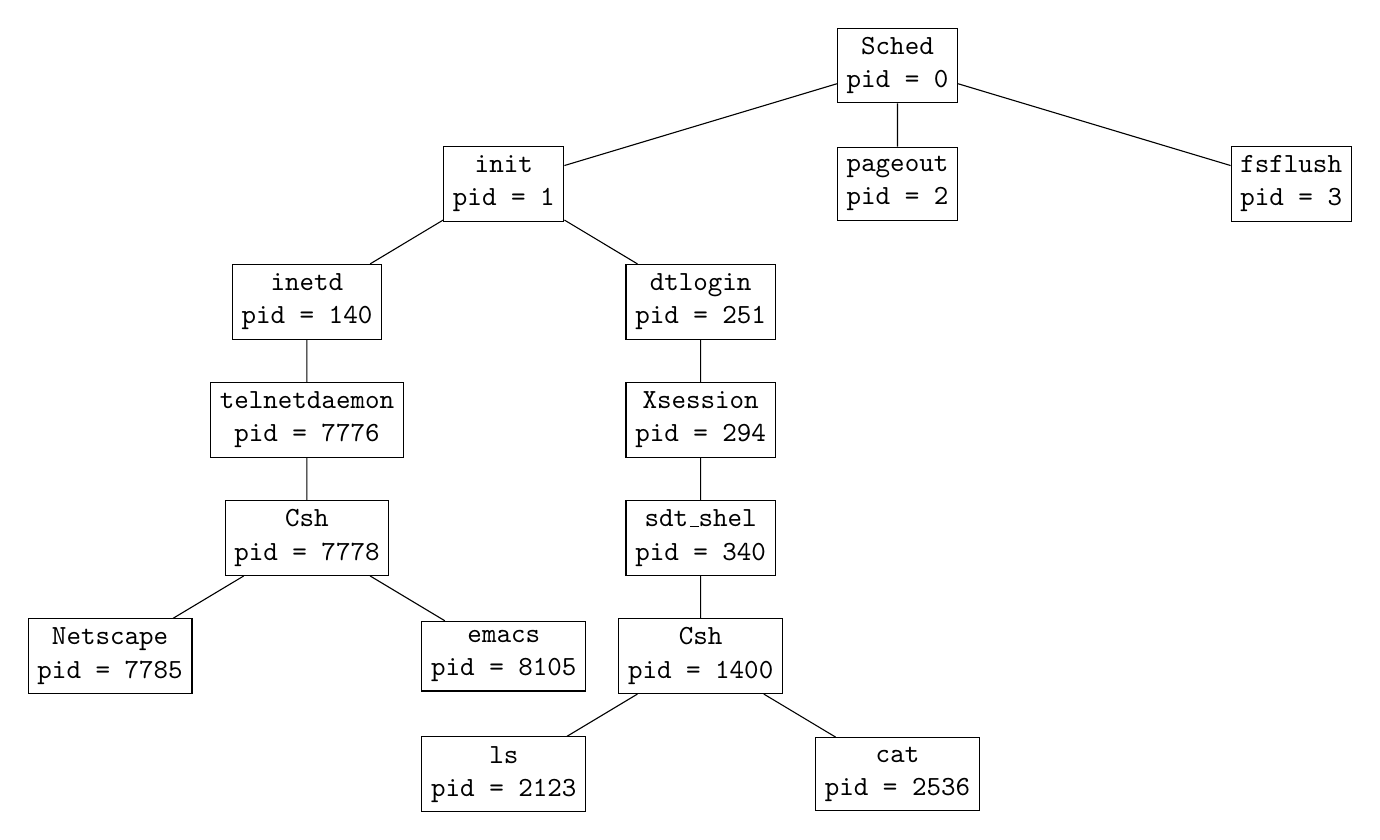
\begin{tikzpicture}[sibling distance = 5cm, every node/.style = { draw, rectangle, align = center }]
						\node {\texttt{Sched} \\ \texttt{pid = 0}}
						child { node {\texttt{init} \\ \texttt{pid = 1}}
							child { node {\texttt{inetd} \\ \texttt{pid = 140}}
								child { node {\texttt{telnetdaemon} \\ \texttt{pid = 7776}}
									child { node {\texttt{Csh} \\ \texttt{pid = 7778}}
										child { node {\texttt{Netscape} \\ \texttt{pid = 7785}} }
										child { node {\texttt{emacs} \\ \texttt{pid = 8105}} } } } }
							child { node {\texttt{dtlogin} \\ \texttt{pid = 251}}
								child { node {\texttt{Xsession} \\ \texttt{pid = 294}}
									child { node {\texttt{sdt\_shel} \\ \texttt{pid = 340}}
										child { node {\texttt{Csh} \\ \texttt{pid = 1400}}
											child { node {\texttt{ls} \\ \texttt{pid = 2123}} }
											child { node {\texttt{cat} \\ \texttt{pid = 2536}} } } } } } }
						child { node {\texttt{pageout} \\ \texttt{pid = 2}} }
						child { node {\texttt{fsflush} \\ \texttt{pid = 3}} };
					\end{tikzpicture}
					\caption{Process Tree: Solaris}
				\end{figure}
				% end
				% end
				% end

	\section{Concurrency}
		\begin{itemize}
			\item If more processes than CPUs exist, the processes must be executed \textit{concurrently}. There are multiple mechanisms for concurrent execution:
				\begin{enumerate}
					\item One after another
					\item Interleaved execution
				\end{enumerate}
			\item All these mechanisms need that
				\begin{itemize}
					\item switching between processes is possible and that
					\item switching does not operations of a process.
				\end{itemize}
		\end{itemize}
		% end

	\section{Process Management}
		Process management includes the following steps:
		\begin{enumerate}
			\item Running, suspending and resuming processes
			\item Process creation
			\item Process termination
			\item Provide inter-process communication (IPC) for cooperating processes
		\end{enumerate}
		This needs scheduling, synchronization and deadlock handling for all processes.

		During the execution of a process, the process runs through multiple "process states":
		\begin{figure}[H]
			\centering
			\begin{tikzpicture}[state/.style = { draw, rectangle, minimum height = 0.8cm, minimum width = 2.5cm }]
				\node [state] (new) {new};
				\node [state, yshift = -1cm, below right = 1 of new] (ready) {ready};
				\node [state, yshift = -1cm, below right = 1 of ready] (waiting) {waiting};
				\node [state, yshift = 1cm, above right = 1 of waiting] (running) {running};
				\node [state, yshift = 1cm, above right = 1 of running] (terminated) {terminated};

				\path (ready.north east) -- coordinate(a) (ready.east);
				\path (ready.south east) -- coordinate(b) (ready.east);
				\path (running.north west) -- coordinate(c) (running.west);
				\path (running.south west) -- coordinate(d) (running.west);

				\draw [->] (b) -- node[below]{schedule} (d);
				\draw [->] (c) -- node[above]{deschedule} (a);

				\draw [->] (new) |- node[left]{admit} (ready);
				\draw [->] (waiting) -| node[left]{I/O, event wait finish} (ready);
				\draw [->] (running) |- node[right]{I/O, event wait} (waiting);
				\draw [->] (running) -| node[right]{exit} (terminated);
			\end{tikzpicture}
			\caption{Process States}
		\end{figure}
		\begin{description}
			\item[new] Process initialized
			\item[ready] Waiting for CPU assignment
			\item[running] Instructions are executed
			\item[waiting] Waiting for I/O or events
			\item[terminated] Finished execution
		\end{description}

		\subsection{Process Control Block}
			\begin{itemize}
				\item Essential for switching between processes.
				\item Saves the context for a processes to survive the switch. The context contains:
					\begin{itemize}
						\item Which instruction was executing (PC)
						\item What is was doing (register contents)
						\item Which resources where used (memory, I/O)
					\end{itemize}
				\item The context switch is "overhead" on both OS and HW as the system does not do useful work while switching.
			\end{itemize}

			The PCB is used like this:
			\begin{figure}[H]
				\centering
				\begin{tikzpicture}[action/.style = { draw, rectangle }]
					\node (p0) {Process \(P_0\)};
					\node [right = 2 of p0] (os) {Operating System};
					\node [right = 2 of os] (p1) {Process \(P_1\)};

					\coordinate [below = 0.5 of p0] (a0);
					\coordinate [below = 1 of a0] (a1);
					\coordinate [left = 0.1 of a1] (a1a);
					\coordinate [right = 0.1 of a1] (a1b);
					\coordinate [below = 0.5 of os] (b0);
					\path let \p1 = (a1), \p2 = (b0) in coordinate (b1N) at (\x2, \y1);
					\coordinate [below = 0.5 of b1N] (b1);
					\node [action, below = 0 of b1] (b2) {save state into \(\textrm{PCB}_0\)};
					\node [below = 0 of b2] (b3) {\(\vdots\)};
					\node [action, below = 0.14 of b3] (b5) {reload state from \(\textrm{PCB}_1\)};
					\coordinate [below = 0.5 of b5] (b4);
					\coordinate [below = 0.5 of p1] (c0);
					\path let \p1 = (b4), \p2 = (c0) in coordinate (c1) at (\x2, \y1);
					\coordinate [left = 0.1 of c1] (c1a);
					\coordinate [right = 0.1 of c1] (c1b);
					\coordinate [below = 3 of c1] (c2);
					\coordinate [left = 0.1 of c2] (c2a);
					\coordinate [right = 0.1 of c2] (c2b);
					\path let \p1 = (c2), \p2 = (b0) in coordinate (b6N) at (\x2, \y1);
					\coordinate [below = 0.5 of b6N] (b6);
					\node [action, below = 0 of b6] (b7) {save state into \(\textrm{PCB}_1\)};
					\node [below = 0 of b7] (b8) {\(\vdots\)};
					\node [action, below = 0.14 of b8] (b10) {reload state from \(\textrm{PCB}_0\)};
					\coordinate [below = 0.5 of b10] (b9);
					\path let \p1 = (b9), \p2 = (a0) in coordinate (a2) at (\x2, \y1);
					\coordinate [left = 0.1 of a2] (a2a);
					\coordinate [right = 0.1 of a2] (a2b);
					\coordinate [below = 1 of a2] (a3);
					\path let \p1 = (a3), \p2 = (c0) in coordinate (c3) at (\x2, \y1);

					\node [above = 0.5 of b1] {interrupt or system call};
					\node [above = 0.5 of b6] {interrupt or system call};
					\draw [->, line width = 2pt, shorten >= 1pt] (a0) -- node[left]{executing} (a1);
					\draw (a1a) -- (a1b);
					\draw [->, shorten <= 0.2cm] (a1) -| (b1);
					\draw [->, shorten >= 0.2cm] (b5) |- (c1);
					\draw (c0) -- node[right]{idle} (c1);
					\draw (c1a) -- (c1b);
					\draw [->, line width = 2pt, shorten <= 2pt, shorten >= 1pt] (c1) -- node[right]{executing} (c2);
					\draw (c2a) -- (c2b);
					\draw [->, shorten <= 0.2cm] (c2) -| (b6);
					\draw [->, shorten >= 0.2cm] (b10) |- (a2);
					\draw (a2a) -- (a2b);
					\draw [->, line width = 2pt, shorten <= 2pt] (a2) -- node[left]{executing} (a3);
					\draw (a1) -- node[left]{idle} (a2);
					\draw (c2) -- node[right]{idle} (c3);
				\end{tikzpicture}
				\caption{Process Control Block: Usage}
			\end{figure}
			% end

		\subsection{Process Creation (POSIX)}
			\begin{figure}[H]
				\centering
				\begin{tikzpicture}
					\node (fork) {\texttt{fork()}};
					\node [below right = 2 of fork] (exec) {\texttt{exec()}};
					\node [right = 2 of exec] (exit) {\texttt{exit()}};
					\node [above right = 2 of exit] (wait) {\texttt{wait()}};
					\coordinate [right = 2.5 of wait] (end);

					\draw [->] (fork) -- node[left, xshift = -0.2cm]{child} (exec);
					\draw [->] (exec) -- (exit);
					\draw [->] (exit) -- (wait);
					\draw [->] (fork) -- node[above]{parent} (wait);
					\draw [->] (wait) -- node[above]{resumes} (end);
				\end{tikzpicture}
				\caption{POSIX Process Creation}
			\end{figure}
			\begin{itemize}
				\item The \texttt{fork} system call create a new (clone) process.
				\item The \texttt{exec} method is called after \texttt{fork} to replace the memory space with a new program.
				\item The parent \texttt{wait}s until the child finished the execution.
			\end{itemize}

			\paragraph{Example: Forking in C}
				\begin{figure}[H]
					\centering
					\lstinputlisting[language = C]{\lstbasepath/code/fork.c}
					\caption{Forking a Process in C (POSIX)}
				\end{figure}
				% end
				% end

		\subsection{Process Termination}
			\begin{itemize}
				\item A process executes the last statement and asks the OS to delete it (\texttt{exit()}).
					\begin{itemize}
						\item Returns a status value to the parent (via \texttt{wait()}).
						\item The resources of the process are deallocated by the OS.
					\end{itemize}
				\item The parent may terminate the execution of children processes (\texttt{kill()}, \texttt{TerminateProcess()}) if:
					\begin{itemize}
						\item Child has exceeded allocated resources,
						\item task assigned to the child is no longer required or
						\item parent is exiting (some OS do not allow children to continue if the parent terminates (zombie control) \(\rightarrow\) cascading termination).
					\end{itemize}
			\end{itemize}
			% end

		\subsection{Inter-Process-Communication}
			\begin{itemize}
				\item Processes may be
					\begin{itemize}
						\item \textbf{Independent}
							\begin{itemize}
								\item A process is independent if it cannot affect or be affected by other processes executing in the system.
								\item Independent processes do not share data with any other process.
							\end{itemize}
						\item \textbf{Cooperating}
							\begin{itemize}
								\item A process is cooperating if it can affect or be affected by other processes executing in the system.
								\item Cooperating processes share data with any other process.
							\end{itemize}
					\end{itemize}
				\item Cooperating processes are needed for information sharing, speedup, modularity, privilege separation, etc.
				\item But this brings up a few issues:
					\begin{itemize}
						\item Data sharing
						\item Processes need a communication channel or medium
						\item Coordinate and synchronization (race conditions, deadlocks; critical sections, locking, semaphores, see \ref{c:deadlocks}, \ref{c:scheduling} and \ref{c:mutualexclusion}).
					\end{itemize}
			\end{itemize}
			% end
			% end

	\section{Inter-Process-Communication Models}
		There are two basic IPC-models:
		\begin{enumerate}
			\item \textit{Shared Memory} \\ Processes use shared memory region as communication medium.
			\item \textit{Message Passing} \\ Processes use (abstract) communication link with primitive operations for sending/receiving messages.
		\end{enumerate}

		\subsection{Shared Memory}
			\begin{itemize}
				\item Cooperating processes:
					\begin{itemize}
						\item \textit{Producer} process produced data items.
						\item \textit{Consumer} process consumes data items.
						\item Both share a memory region named \textit{buffer}.
					\end{itemize}
				\item The buffer can either be bounded with a fixed buffer size or unbounded with no practical limit.
			\end{itemize}

			\paragraph{Example: Bounded Buffer in C}
				\begin{figure}[H]
					\centering
					\begin{lstlisting}[language = C]
// Buffer boundary (ten items).
#define BUFFER_SIZE = 10

typedef struct { ... } item;

// Shared circular buffer.
item buffer[BUFFER_SIZE];
// Next free position, shared.
int in = 0;
// First full position, shared.
int out = 0;
\end{lstlisting}
					\caption{Bounded Buffer in C}
				\end{figure}
				\begin{itemize}
					\item The buffer is empty if and only if \lstinline[language = C]|in == out| holds.
					\item The buffer is full if and only if \lstinline[language = C]|(in + 1) % BUFFER_SIZE == out| holds.
				\end{itemize}

				\begin{figure}[H]
					\centering
					\begin{lstlisting}[language = C]
// Producer: Waits if buffer is full and inserts new items.
while (1) {
	// Do nothing, buffer is full.
	while ((in + 1) % BUFFER_SIZE == out) { }

	// Produce a new item and place it in the buffer.
	buffer[in] = new_item;
	in = (in + 1) % BUFFER_SIZE;
}
\end{lstlisting}
					\caption{Bounded Buffer in C: Producer}
				\end{figure}

				\begin{figure}[H]
					\centering
					\begin{lstlisting}[language = C]
// Consumer: Waits if buffer is empty and removes items.
while (1) {
	// Do nothing, buffer is empty.
	while (in == out) { }

	// Remove an item from the buffer and process it.
	current_item = buffer[out];
	out = (out + 1) % BUFFER_SIZE;
	process(current_item);
}
\end{lstlisting}
					\caption{Bounded Buffer in C: Consumer}
				\end{figure}
				% end
				% end

		\subsection{Message Passing}
			\begin{itemize}
				\item Processes use two primitive operations for sending/receiving messages (with either a fixed or variable size).
					\begin{itemize}
						\item \texttt{send(message)}
						\item \texttt{receive(message)}
					\end{itemize}
				\item If two processes (say \(P\) and \(Q\)) want to communicate, they need to establish a \textit{communication link} and exchange messages via send/receive.
				\item The implementation and design of the communication link may either be physical (hardware bus, network, \dots) or logical (software abstractions, \dots).
				\item The implementation leads to the following issues that have to be taken care of:
					\begin{itemize}
						\item How to establish the link?
						\item Can the link be associated with more than two processes?
						\item How many links exist between every pair of processes?
						\item What is the capacity of a link?
						\item Is the size of a message fixed or variable?
						\item Is a link unidirectional or bidirectional?
						\item[\(\rightarrow\)] Addressing, naming (direct vs. indirect)
						\item[\(\rightarrow\)] Synchronization aspects (blocking vs. nonblocking)
						\item[\(\rightarrow\)] Buffering (link capacity)
					\end{itemize}
			\end{itemize}

			\subsubsection{Addressing}
				\begin{itemize}
					\item The communicating processes need to name each other explicitly:
						\begin{itemize}
							\item \(P\): \texttt{send(Q, msg)} (Process \(P\) sends a message to process \(Q\))
							\item \(Q\): \texttt{receive(P, msg)} (Process \(Q\) receives a message from process \(P\))
						\end{itemize}
					\item The addressing can take place symmetric or asymmetric, where the latter means that one process "listens" for other processes and then stores the corresponding PID (Process ID) for sending messages back.
						\begin{description}
							\item[symmetric] \texttt{send(Q, msg)}; \texttt{receive(P, msg)}
							\item[asymmetric] \texttt{send(Q, msg)}; \texttt{receive(\&pid, msg)}
						\end{description}
					\item Using indirect communication, messages are directed to and received from \textit{mailboxes} or \textit{ports}.
						\begin{itemize}
							\item The communicating processes to not have to know the name of each other.
							\item Each mailbox has its unique ID and can be used for send/receive.
							\item Processes can only communicate if they share a mailbox.
							\item Example: UNIX pipes like \texttt{cat xzy | lpr} (implicit FIFO mailbox).
						\end{itemize}
				\end{itemize}
				% end

			\subsubsection{Synchronization}
				\begin{itemize}
					\item Message passing may either be \textit{blocking} or \textit{nonblocking}.
					\item \textit{Blocking} (B) is considered synchronous:
						\begin{itemize}
							\item \texttt{B.Send} The sender blocks until the message was received.
							\item \texttt{B.Receive} The receiver blocks until a message is available.
							\item \texttt{Rendezvous} Both sender and receive are blocking.
						\end{itemize}
					\item \textit{Nonblocking} (NB) is considered asynchronous:
						\begin{itemize}
							\item \texttt{NB.Send} The sender sends the message and continues.
							\item \texttt{NB.Receive} The receive receives a valid message or nothing (null).
						\end{itemize}
				\end{itemize}
				% end

			\subsubsection{Message Buffering (Queues)}
				The messages reside in temporary queues that can be implemented in one of three possible ways:
				\begin{itemize}
					\item \textit{Zero capacity} - no messages can be stored \\ The sender must wait for the receiver for each message (rendezvous).
					\item \textit{Bounded capacity} - finite length of \(n\) messages can be stored \\ The sender must only wait if the queue is full.
					\item \textit{Unbounded capacity} - infinite length \\ The sender never waits.
				\end{itemize}
				% end

			\subsubsection{Pipes}
				\begin{itemize}
					\item \textit{Pipes} are conduits that allow two processes to communicate.
					\item Implementation issues:
						\begin{itemize}
							\item Provide uni- or bidirectional communication?
							\item What is the relationship between communicating processes (parent/child)?
						\end{itemize}
					\item An ordinary (anonymous) pipe is:
						\begin{itemize}
							\item Unidirectional,
							\item creates using the \texttt{pipe()} system call,
							\item is not accessible outside of the creating process and
							\item creates two files descriptors:
								\begin{itemize}
									\item \texttt{fd[0]}: read-end
									\item \texttt{fd[1]}: write-end
								\end{itemize}
						\end{itemize}
				\end{itemize}
				% end

			\subsubsection{Example: (A)LPC in Windows}
				\begin{figure}[H]
					\centering
					\begin{tikzpicture}[handle/.style = { minimum height = 7cm, minimum width = 2cm }, main/.style = { draw, rectangle }, every node/.style = { minimum height = 0.8cm }]
						\node [main, handle, label = above:Client] (client) {Handle};
						\path (client.north east) -- coordinate(a) (client.east);
						\path (client.south east) -- coordinate(b) (client.east);
						\node [main, right = 1 of client.east] (comClient) {Com. port: Client};
						\node [main, right = 1 of comClient] (comServer) {Com. port: Server};
						\node [main, handle, anchor = west, right = 1 of comServer, label = above:Server] (server) {Handle};
						\path (server.north west) -- coordinate(A) (server.west);
						\path (server.south west) -- coordinate(B) (server.west);

						\path (a) -- node[main](c){Conn. port} (A);
						\path (b) -- node[main, label = below:{(Used for large messages)}](d){Shared section object} (B);

						\draw [->] (a) -- node[above]{Conn. req.} (c);
						\draw [->] (c) -- node[above]{Handle} (A);

						\draw [<->] (b) -- (d);
						\draw [<->] (d) -- (B);

						\draw [->] (comClient) -- (client);
						\draw [->] (comServer) -- (server);

						\path (comClient.north east) -- coordinate(x) (comClient.east);
						\path (comClient.south east) -- coordinate(z) (comClient.east);
						\path (comServer.north west) -- coordinate(X) (comServer.west);
						\path (comServer.south west) -- coordinate(Z) (comServer.west);

						\draw [->] (x) -- (X);
						\draw [<-] (z) -- (Z);
					\end{tikzpicture}
					\caption{(A)LPC in Windows}
				\end{figure}

				\begin{enumerate}
					\item The client opens a handle to the connection port object of the subsystem.
					\item The client sends a communication request.
					\item The server creates two private communication ports and returns the handle to the client.
					\item The client and the server use the corresponding port handle to send messages (and callback to listen for replies).
				\end{enumerate}
				% end
				% end
				% end
				% end

\chapter{Threads}
	\begin{itemize}
		\item Programs often perform multiple tasks concurrently (writing data to disk, perform spell checking, \dots).
		\item Problematic: Using separate processes with IPC is cumbersome and has lots of performance drawbacks.
		\item Solution: Allow processes to have multiple \textit{threads} executing concurrently for different tasks.
		\item Benefits of multithreading:
			\begin{enumerate}
				\item \textbf{Responsiveness} \\ Allows a program to continue even if other parts of the program are blocked.
				\item \textbf{Resource Sharing} \\ Threads share process resources which is easier than explicit IPC.
				\item \textbf{Efficiency/Performance} \\ Creating and context switching of threads produced a lot less work than for processes.
				\item \textbf{Scalability} \\ Processes can take advantage of multiprocessor architectures and worker threads can be dispatched to different processors.
			\end{enumerate}
	\end{itemize}

	\section{Process vs. Thread Model}
		\begin{itemize}
			\item \textbf{Process Model} (heavyweight single thread)
				\begin{itemize}
					\item Each process has a discrete and distinct control flow and
					\item unique PC, SP, registers and address space.
					\item The processes interact via IPC.
				\end{itemize}
			\item \textbf{Thread Model} (lightweight sub-processes)
				\begin{itemize}
					\item Each thread runs independently and sequentially and has its own PC and SP like a process.
					\item Each thread can create sub-threads, can request services and has a "state" (ready, running, blocked) like a process.
					\item Difference to processes: All threads of a process share the same address space as the parent process:
						\begin{itemize}
							\item access to global variables within the process
							\item access to all files within the shared address space
							\item reading, writing, deleting variables, files, stacks, \dots
						\end{itemize}
					\item Therefore, threads are much faster and provide concurrency, but there is no isolation between them.
					\item The speedup is best when all threads use different resources (e.g. first one uses the CPU, the second the I/O (keyboard, display, \dots) and the third uses the storage).
				\end{itemize}
		\end{itemize}
		% end

	\section{Example: Multi-Threaded Web Server}
		\begin{itemize}
			\item The request handling is decoupled from the request execution.
			\item The so-called \textit{dispatcher thread} creates a new \textit{worker thread} for each incoming request that then handles the request execution.
			\item With this method the web server is sped up as the requests can be handled concurrently.
			\item This multi-process/child model would also work with processes, however that produces a lot of overload due to process creation, context switching, scheduling, etc.
		\end{itemize}
		% end

	\section{Theoretical Speedup (Amdahl's Law)}
		Amdahl's Law describes the \textit{theoretical speedup} from adding CPUs to programs with parallelized parts.

		Let \(S\) be the serial portion (percentage runtime) and \(N\) the parallel processing cores. Then the formula is:
		\begin{equation*}
			\textit{speedup} \leq \frac{1}{S + \frac{1 - S}{N}} \qquad\qquad \lim\limits_{N \rightarrow \infty} \textit{speedup} = \frac{1}{S}
		\end{equation*}
		% end

	\section{Implementations}
		\begin{itemize}
			\item \textbf{User-Level}
				\begin{itemize}
					\item[+] Each process can define its own thread policies.
					\item[+] Flexible localized scheduling
					\item[--] No kernel knowledge and therefore no kernel support for thread management.
				\end{itemize}
			\item \textbf{Kernel-Level}
				\begin{itemize}
					\item[+] Single thread table under kernel control.
					\item[+] Full kernel overview and thread management.
				\end{itemize}
			\item \textbf{Hybrid}
				\begin{itemize}
					\item Multiplexing of user-level threads onto kernel-level threads.
					\item Each kernel thread owns a limited sphere of user-level threads.
				\end{itemize}
		\end{itemize}

		\subsection{Many-to-One}
			\begin{itemize}
				\item Many user-level threads map onto a single kernel thread.
				\item One thread blocking is causing all other threads to also block.
				\item Multiple threads may not run in parallel because only one is in the kernel at a time.
				\item Examples: Solaris Green Threads, GNU Portable Threads
				\item Pros/Cons
					\begin{itemize}
						\item[+] Flexible as thread management is in user space.
						\item[--] The process blocks if a thread blocks.
						\item[--] Only one thread can access the kernel at a time \(\rightarrow\) no multiprocess support.
					\end{itemize}
			\end{itemize}
			% end

		\subsection{One-to-One}
			\begin{itemize}
				\item Each user-level thread maps onto a kernel thread.
				\item Creating user-level threads results in creating a kernel thread.
				\item More concurrency than many-to-one.
				\item The number of threads per process is sometimes restricted due to overhead.
				\item Examples: Windows, Linux; Solar 9+
			\end{itemize}
			% end

		\subsection{Many-to-Many}
			\begin{itemize}
				\item Many user.level threads map onto many kernel threads.
				\item Allows the OS to create a sufficient number of kernel threads.
				\item Examples: Solaris prior version 9, Windows Fibers
				\item Pros/Cons
					\begin{itemize}
						\item[+] Large number of threads.
						\item[+] If the user-thread blocks, the kernel schedules another for execution.
						\item[--] Less concurrency than one-to-one mapping.
					\end{itemize}
			\end{itemize}
			% end

		\subsection{Two-level Model}
			\begin{itemize}
				\item Similar to many-to-many, except that it allows that a user-level thread is bound to a kernel thread.
				\item Examples: IRIX, HP-UX, Tru64 UNIX, Solaris prior to version 8
			\end{itemize}
			% end
			% end

	\section{Linux Threads/Tasks}
		\begin{itemize}
			\item Linux calls threads \textit{tasks}.
			\item Linux does not distinguish between processes and threads.
			\item Thread creation is done using \texttt{clone()} system call with flags indicating the sharing method.
			\item \texttt{clone()} allows a child task to share the address space/file descriptors/signals of the parent task with the following flags:
		\end{itemize}
		\begin{table}[H]
			\centering
			\begin{tabular}{c | c}
				Flag                    & Meaning                        \\ \hline
				\texttt{CLONE\_FS}      & Share file-system information. \\
				\texttt{CLONE\_VM}      & Share memory address space.    \\
				\texttt{CLONE\_SIGHAND} & Share signal handlers.         \\
				\texttt{CLONE\_FILES}   & Share set of open files
			\end{tabular}
			\caption{Linux: Possible \texttt{clone()} flags}
		\end{table}
		\begin{itemize}
			\item \texttt{struct task\_struct} points to the data structures of the process.
			\item Both functions \texttt{pthread\_create()} and \texttt{fork()} are implemented using \texttt{clone()}.
		\end{itemize}
		% end

	\section{POSIX Threads (C)}
		\begin{figure}[H]
			\centering
			\begin{lstlisting}[language = C]
int result = 0;

void* thread_func(void* arg) {
	for (int i = 0; i < MAX; ++i) {
		result += 42;
	}
	return NULL;
}

int main() {
	// Stores the thread ID (TID) for later communication.
	pthread_t tid;
	pthread_create(&tid, NULL, thread_func, NULL);
	...
	// Wait until the thread is finished.
	pthread_join(tid, NULL);
	printf("Result: %d\n", result);
	return 0;
}
\end{lstlisting}
			\caption{POSIX Threads in C}
		\end{figure}
		% end

	\section{Single to Multi-Threaded}
		\begin{itemize}
			\item If multiple threads access the same global variable at once, the changes of one of the threads may be lost.
			\item This problem can be solved by allowing threads to have a private copy of the global variables (thread-local storage, TLS).
			\item The TLS therefore keeps a private copy of the global variables.
		\end{itemize}
		% end
		% end

\chapter{Deadlocks and Resource Management}
	\label{c:deadlocks}

	\section{Resource Management}
		\begin{itemize}
			\item The number of resources in a system is finite, but there are lots or processes created by the OS.
			\item The OS has to manage the resources addressing:
				\begin{itemize}
					\item Resource constraints
					\item Ordering of processes, IPC
					\item Precedence relations
					\item Access control for global parameters
					\item Shared memory
					\item Scheduling
					\item and so on\dots
				\end{itemize}
				This solutions must be \textit{fair}, \textit{efficient}, \textit{deadlock-free} and \textit{race-free}.
		\end{itemize}

		\subsection{Google Chubby Lock Service}
			\textit{Google Chubby} is a distributed lock service developed by Google to synchronize Client/Server interactions and accesses to shared resources. It is used by a lot of the infrastructure of Google (GFS, BigTable, MapReduce, \dots).

			Problems:
			\begin{itemize}
				\item One node is holding a consistency lock that others need to access to proceed. Therefore, if one node holding lock hangs, the client/server hangs.
				\item Multiple locks get set; old lock is not released leads to inconsistent masters.
				\item If server partitions happen, the resource access is inconsistent and R/W data consistency is lost.
			\end{itemize}
			% end

		\subsection{Resource Sharing and Inter-Process-Interaction}
			The ordering of processes/threads for handling resource contentions include the following points to consider:
			\begin{itemize}
				\item What to do if a process starts writing to a section that another process is currently reading?
				\item What to do if a new process gets allocated the same resource already allocated to an existing process?
				\item What to do if a slow/stalled process blocks other processes from executing?
				\item \dots
			\end{itemize}
			All in all this can be concluded as: How to have a shared resource (\textit{critical section}, \textit{CS}) be allocated by only one process at a time (\textit{mutually exclusive access}, \textit{ME}) such that the outcome is of a correctly ordered execution?

			\subsubsection{Mutual Exclusion}
				See \ref{c:mutualexclusion}.
				% end
				% end
				% end

	\section{Deadlock/Livelock and Starvation}
		A set of processes is deadlocked if every process waits for a resources held by another process.
		\begin{description}
			\item[Deadlock] None of the processes can be run, releases or be awakened.
			\item[Livelock] All processes (can be) run, but no progress is made (e.g. because of missing data of another process).
		\end{description}
		% end

	\section{Deadlock Conditions}
		For a deadlock to be possible, all of the following conditions have to be fulfilled:
		\begin{description}
			\item[Mutual Exclusion] Each resource has to be accessed mutually exclusive.
			\item[Hold and Wait] A process holding at least one resource has requested and is waiting to acquire additional resourced currently held by another process.
			\item[No Preemption] A resource cannot be acquired forcibly from a process holding it. It can only be release if the holding process releases it voluntarily after the process has completed its task.
			\item[Circular Wait] A circular chain of more than one process exists. Let \( \{ P_0, P_1, \cdots, P_n, P_0 \} \) be a chain of waiting processes where each process \( P_i \) waits for a resource held by \( P_{ (i + 1) \textbf{ mod } n } \) (forming a dependency cycle).
		\end{description}
		If either of these conditions is not given, no deadlock can occur.
		% end

	\section{Deadlock Modeling and Visualization}
		Deadlocks (more specifically resource dependencies) can be visualized as graphs (where circles are processes and rectangles resources):
		\begin{figure}[H]
			\centering
			\begin{tikzpicture}[every node/.style = { minimum height = 0.8cm, minimum width = 0.8cm }]
				\node [shape = circle, draw, inner sep = 2pt] (a1) {A};
				\node [below = 2 of a1, draw, rectangle] (r1) {R};
				\node [right = 3 of r1, shape = circle, draw, inner sep = 2pt] (a2) {A};
				\node [right = 3 of a1, draw, rectangle] (s1) {S};

				\draw [->] (r1) -- node[left]{has} (a1);
				\draw [->] (a2) -- node[left]{needs} (s1);
			\end{tikzpicture}
			\caption{Deadlock Modeling: Graphs}
		\end{figure}

		\begin{figure}[H]
			\centering
			\begin{tikzpicture}[process/.style = { shape = circle, draw, inner sep = 2pt }, resource/.style = { draw, rectangle }, every node/.style = { minimum height = 0.8cm, minimum width = 0.8cm }]
				\coordinate (center) at (0, 0);
				\node [process, above = 1 of center] (a) {A};
				\node [process, below = 1 of center] (b) {B};
				\node [resource, right = 1 of center] (s) {S};
				\node [resource, left = 1 of center] (r) {R};

				\draw [->] (a.east) to[bend left, out = 45, in = 135] node[right, xshift = 0.1cm]{needs} (s.north);
				\draw [->] (s.south) to[bend left, out = 45, in = 135] node[right, xshift = 0.1cm]{has} (b.east);
				\draw [->] (b.west) to[bend left, out = 45, in = 135] node[left, xshift = -0.1cm]{needs} (r.south);
				\draw [->] (r.north) to[bend left, out = 45, in = 135] node[left, xshift = -0.1cm]{has} (a.west);
			\end{tikzpicture}
			\caption{Example: Deadlock Modeling: Graph}
		\end{figure}

		Using graphs, it is extremely simple to spot cycles. These cycles can be removed by reordering the requests, but:
		\begin{itemize}
			\item Requests are often dynamic/streaming,
			\item The OS has no global overview and
			\item Tasks have precedence relations, priorities, timing duration, etc.
		\end{itemize}
		So this is a very hard task. This task is implemented by \textit{ordering and scheduling algorithms}.
		% end

	\section{Deadlock Strategies}
		There are three general strategies for dealing with deadlock:
		\begin{itemize}
			\item \textbf{Ignore} the problem (it might just go away)
				\begin{itemize}
					\item Implemented by Windows, UNIX, \dots
					\item It works, iff:
						\begin{itemize}
							\item The cost (in terms of workload) for avoidance/prevention is high.
							\item Deadlocks occur rarely enough or may possibly go away with random/exponential back-offs (timeouts) on service responses.
						\end{itemize}
					\item Using this method, there is a trade-off between convenience (cost, complexity, \dots) and correctness (repeatability, predictability, \dots).
				\end{itemize}
			\item \textbf{Detect} and \textbf{Recover} (check, detect, recover)
			\item \textbf{Avoid} and \textbf{Prevent} (by design, negate one of the four conditions for deadlocks)
		\end{itemize}

		\subsection{Detection}
			\begin{itemize}
				\item Every OS has a "resource allocation checker" that performs static tests for deadlocks.
				\item Dynamic checking may vary from rigid/static processes to heuristic/adaptive tests.
			\end{itemize}

			\subsubsection{One Resource per Type}
				\begin{itemize}
					\item Develop resource ownership and requests graph.
					\item If a cycle is found, this indicates a deadlock.
					\item[\(\rightarrow\)] Set up a DS (depth search, e.g. a spanniong) where a cycle is visible via node repetition in the DS. A spanning tree is a subset of the edges of a graph connecting all edges without any cycles.
				\end{itemize}
				% end

			\subsubsection{Multiple Resources per Type}
				\label{sec:deadlockdetection}

				\begin{itemize}
					\item Spanning tree computation is hard, so for multiple types, a simple matrix data structure is more convenient.
				\end{itemize}

				Let \( E = (E_1, \cdots, E_n)^T \) be the vector of all \textit{existing} resources of the resource types \( R_1, \cdots, R_n \). Let \( A = (A_1, \cdots, A_n)^T \) be the vector of \textit{remaining} resources of the resource types. Notice that in any state, the formula \( A_i \leq R_i \) holds true for every \(i\). Using this lets define matrices \( Q \in \mathbb{N}_0^{n \times m} \) and \( T \in \mathbb{N}_0^{n \times m} \) where \(Q\) represents, which process (of a set of processes \( \{ P_1, \cdots, P_m \} \)) holds how many resources of each type (the entry \( Q_{ij} \) indicates how many resources of type \( R_j \) the process \( P_i \) holds). Furthermore, the matrix \(T\) defines (in a similar way) which process requested how many resources of each time. Notice that in any state, the formula \( \sum_{i = 1}^{n} C_{ij} + A_j = E_j \) holds true for every \(j\). A matrix \( R \coloneqq T - Q \) contains the numbers how many resources are still needed (i.e. not yet provided).

				In summary, the vectors and matrices look like this (the rows of the matrices show how many resources the process currently holds/needs):
				\begin{equation*}
					\begin{array}{rclcrcl}
						E                                             & \coloneqq &
						\begin{bmatrix}
							E_1    \\
							\vdots \\
							E_n
						\end{bmatrix}                               & \qquad    &
						A                                             & \coloneqq &
						\begin{bmatrix}
							A_1    \\
							\vdots \\
							A_n
						\end{bmatrix}                                                    \\ \\
						Q                                             & \coloneqq &
						\begin{bmatrix}
							Q_{11} & Q_{12} & Q_{13} & \cdots & Q_{1m} \\
							Q_{21} & Q_{22} & Q_{23} & \cdots & Q_{2m} \\
							\vdots & \vdots & \vdots & \ddots & \vdots \\
							Q_{n1} & Q_{n2} & Q_{n3} & \cdots & Q_{nm}
						\end{bmatrix} & \qquad    &
						T                                             & \coloneqq &
						\begin{bmatrix}
							R_{11} & R_{12} & R_{13} & \cdots & R_{1m} \\
							R_{21} & R_{22} & R_{23} & \cdots & R_{2m} \\
							\vdots & \vdots & \vdots & \ddots & \vdots \\
							R_{n1} & R_{n2} & R_{n3} & \cdots & R_{nm}
						\end{bmatrix}                        \\
						R                                             & \coloneqq & T - Q
					\end{array}
				\end{equation*}

				\paragraph{Progress via Process Selection}
					Definition: Let \( a, b \in \mathbb{N}^n \), than \( a \leq b \) hold iff \( a_i \leq b \) for all \( i \).

					If at least one row \(r\) exists in \(R\) with \( r \leq A \), enough resources are available and the process is able to continue. If not, a deadlock \textit{may} occur.
					% end
					% end
					% end

		\subsection{Recovery}
			\begin{itemize}
				\item \textbf{Recovery through preemption}
					\begin{itemize}
						\item Take a resource from an executing process (depending on the nature of the resource and if the process is interruptible).
					\end{itemize}
				\item \textbf{Recovery through rollback or back-offs}
					\begin{itemize}
						\item Periodically create checkpoints.
						\item Use this saved state and restart the process if a deadlock was found.
					\end{itemize}
				\item \textbf{Recovery through killing processes} (Reactive or Proactive)
					\begin{itemize}
						\item Crudest but simplest method to break the deadlock: Kill one on the processes in the deadlock cycle and release its resources.
						\item Choose a process that can be rerun (e.g. from beginning or a checkpoint) and does not hold up other active processes with precedence dependencies.
					\end{itemize}
			\end{itemize}
			% end

		\subsection{Avoidance}
			\begin{itemize}
				\item Assumes a priori resource information.
				\item The simplest and most useful model requires that each process a priori declares the maximum number of resources of each type that it may need.
				\item The deadlock avoidance algorithm then dynamically examines the resource allocation state to ensure that it is not possible to produce a waiting cycle (safe vs. unsafe scenarios).
				\item The resource allocation state is defined by the number of available and allocated resources and the maximum demand of the process.
			\end{itemize}

			\subsubsection{Execution Trajectories} % 4.23, 4.24
				\begin{figure}[H]
					\centering
					\begin{tikzpicture}
						\coordinate [label = above:B] (B) at (0, 8);
						\coordinate [label = below:A] (A) at (7, 0);
						\coordinate [label = below:p] (p) at (0, 0);
						\coordinate [label = below:q] (q) at (1, 0);
						\coordinate [label = above left:r] (r) at (1, 2);
						\coordinate [label = below:s] (s) at (2.5, 2);
						\coordinate [label = above:t] (t) at (2.5, 3);
						\coordinate [label = below right:u] (u) at (5, 3);
						\coordinate [label = above left:v] (v) at (5, 8);
						\coordinate [label = above right:{w (both finished)}] (w) at (7, 8);

						\coordinate (i1) at (2, 0);
						\coordinate (i2) at (3, 0);
						\coordinate (i3) at (4, 0);
						\coordinate (i4) at (5, 0);

						\coordinate (i5) at (0, 3);
						\coordinate (i6) at (0, 4);
						\coordinate (i7) at (0, 5);
						\coordinate (i8) at (0, 6);

						\coordinate [below = 0.5 of i1] (printerAs);
						\coordinate [below = 0.5 of i3, label = right:Printer] (printerAe);
						\coordinate [below = 1 of i2, label = left:Plotter] (plotterAs);
						\coordinate [below = 1 of i4] (plotterAe);

						\coordinate [left = 0.5 of i5, label = below left:Plotter] (printerBs);
						\coordinate [left = 0.5 of i7] (printerBe);
						\coordinate [left = 1 of i6] (plotterBs);
						\coordinate [left = 1 of i8, label = above left:Printer] (plotterBe);

						\coordinate [above = 0.2 of printerAe] (needle1);
						\coordinate [below = 0.2 of printerAe] (needle2);
						\coordinate [above = 0.2 of printerAs] (needle3);
						\coordinate [below = 0.2 of printerAs] (needle4);
						\coordinate [above = 0.2 of plotterAe] (needle5);
						\coordinate [below = 0.2 of plotterAe] (needle6);
						\coordinate [above = 0.2 of plotterAs] (needle7);
						\coordinate [below = 0.2 of plotterAs] (needle8);

						\draw (needle1) -- (needle2);
						\draw (needle3) -- (needle4);
						\draw (needle5) -- (needle6);
						\draw (needle7) -- (needle8);

						\coordinate [left  = 0.2 of printerBe] (needle1);
						\coordinate [right = 0.2 of printerBe] (needle2);
						\coordinate [left  = 0.2 of printerBs] (needle3);
						\coordinate [right = 0.2 of printerBs] (needle4);
						\coordinate [left  = 0.2 of plotterBe] (needle5);
						\coordinate [right = 0.2 of plotterBe] (needle6);
						\coordinate [left  = 0.2 of plotterBs] (needle7);
						\coordinate [right = 0.2 of plotterBs] (needle8);

						\draw (needle1) -- (needle2);
						\draw (needle3) -- (needle4);
						\draw (needle5) -- (needle6);
						\draw (needle7) -- (needle8);

						\draw [step = 1] (0, 0) grid (7, 8);

						\draw [fill = fgcolor] (p) circle (0.1);
						\draw [fill = fgcolor] (q) circle (0.1);
						\draw [fill = fgcolor] (r) circle (0.1);
						\draw [fill = fgcolor] (s) circle (0.1);
						\draw [fill = fgcolor] (t) circle (0.1);
						\draw [fill = fgcolor] (u) circle (0.1);
						\draw [fill = fgcolor] (v) circle (0.1);
						\draw [fill = fgcolor] (w) circle (0.1);

						\draw (p) -- (B);
						\draw (p) -- (A);

						\draw [<->] (printerAs) -- (printerAe);
						\draw [<->] (plotterAs) -- (plotterAe);
						\draw [<->] (printerBs) -- (printerBe);
						\draw [<->] (plotterBs) -- (plotterBe);

						\draw [line width = 2pt, color = TUDa-3a] (2, 4) rectangle (4, 6);
						\draw [step = 0.2, color = TUDa-3a] (2, 4) grid (4, 6);

						\draw [line width = 2pt, color = TUDa-7a] (3, 3) rectangle (5, 5);
						\draw [step = 0.2, color = TUDa-7a] (3, 3) grid (5, 5);

						\draw [line width = 2pt, color = TUDa-9\IfDarkModeTF{a}{b}] (2, 3) rectangle (3, 4);

						\draw [->, line width = 3pt, > = { Latex[length = 10pt] }] (p) -- (q) -- (r) -- (s) -- (t) -- (u) -- (v) -- (w);
					\end{tikzpicture}
					\caption{Example: Execution Trajectories}
				\end{figure}

				\begin{itemize}
					\item This diagram shows the execution trajectory through two processes where either one uses both the printer and the plotter.
					\item The trajectory itself (the \IfDarkModeTF{white}{black} line) is monotonically increasing and represents the execution process in process A (horizontally) and B (vertically).
					\item It cannot enter either one of the hatched fields, because this would require both processes to access the printer (green) or the plotter (orange), which is denied by the mutual exclusivity (ME). Entering these regions would cause a deadlock.
					\item The red marked region is an unsafe state as it is only possible for the trajectory to move onto a deadlock.
				\end{itemize}
				% end

			\subsubsection{Safe/Unsafe States and Execution Orders}
				An execution order is \textit{safe} iff a sequence order exists that satisfies even if all processes request their maximum resources (keeping in mind that only one process can execute at any time).
				% end

			\subsubsection{Banker's Algorithm for a Single Resource}
				If a safe order is possible from the current state, then grant access. Otherwise, deny the request.

				This avoids deadlocks by design by only permitting safe states. In reality, the criteria for credits/loans can be based on:
				\begin{itemize}
					\item the past behavior of the processes, or
					\item bursty traffic analysis (likelihood of run on the bank), or
					\item constrained maxima (this method is the most common, but abused by DoS attacks).
				\end{itemize}
				% end

			\subsubsection{Banker's Algorithm for Multiple Resource}
				This algorithm is based on the matrices defined in \ref{sec:deadlockdetection} and contains the following steps:
				\begin{enumerate}
					\item Look for at least one row in \(R\) that is smaller than or equal to \(A\). If no such row exists, the system is likely to run into a deadlock since no process can finish its task.
					\item Assume that the process of the chosen row requests all the resources it needs and finishes. Mark that process as terminated and add all its resources to \(A\).
					\item Repeat steps 1 and 2 until either all processes are marked as terminated, in which case the initial state was safe, or until a deadlock occurs, in which case it was not.
				\end{enumerate}
				% end
				% end

		\subsection{Prevention}
			Deadlock prevention is about preventing one of the conditions that must hold to allow deadlocks (e.g. by design). That is, "attacking" each of the conditions separately.

			\subsubsection{Attacking the Mutual Exclusion Condition}
				\textbf{Change:} Allow multiple process to access the same resource (via serializers).
				\begin{itemize}
					\item Example: Spooled/buffered printer access via a printer daemon.
						\begin{itemize}
							\item Only the (single) printer daemon actually accesses the printer resource.
							\item Deadlocks for the printer are eliminated.
						\end{itemize}
					\item Problems:
						\begin{itemize}
							\item Not all devices can be spooled.
							\item Not all processes can be buffered and the daemon policy may not support streams.
						\end{itemize}
					\item In general:
						\begin{itemize}
							\item Minimize shared resource assignment.
							\item As few processes as possible actually claim the resource.
						\end{itemize}
				\end{itemize}
				% end

			\subsubsection{Attacking the Hold and Wait Condition}
				\textbf{To break:} Guarantee that whenever a process requests a resource, it does not hold any other resources or a process that is holding a resource does not request more.
				\begin{itemize}
					\item This requires the process to request and be allocated to all its resources before it begins the execution (no wait during the execution), or allow a process to request resources only when the process has none.
						\begin{itemize}
							\item Problem: The OS may not know "all" required resources at the start of run (e.g. in case of dynamic requests).
							\item This ties up resources that other processes could be using \(\rightarrow\) low resource utilization; starvation is possible.
						\end{itemize}
					\item Variation: A process must give up all resources and then request all immediately needed.
				\end{itemize}
				% end

			\subsubsection{Attacking the No Preemption Condition}
				\textbf{Changes:}
				\begin{itemize}
					\item If a process that is holding some resources requests another resource that cannot be immediately allocated to it, then all resources currently held are released.
					\item Preempted resources are added to the list of resources for which the process is waiting.
					\item Processes will be restarted only when it can regain its old resources, as well as the new requested ones.
				\end{itemize}
				\begin{itemize}
					\item It is not always an option to preempt and it depends on the resource and the process type (e.g. when taking away a printer halfway in the job).
				\end{itemize}
				% end

			\subsubsection{Attacking the Circular Wait Condition}
				\textbf{Option 1:} No chain: Processes are entitled to only hold one resource at a time. All processes that request a resource have to give up all other held resources first.
				\begin{itemize}
					\item Problematic Example: If a process wants to copy larges files from memory to printer, it needs two resources \(\rightarrow\) fails.
				\end{itemize}

				\noindent \textbf{Option 2:} Requests are granted in some numerical or precedence sequence (e.g. next request only to a higher numbered resource).
				\begin{itemize}
					\item Low efficiency and long access times; varied resource response characteristics.
					\item High complexity for ordering with large resource set or short request/access patterns.
					\item How to produce consistent numbering across distributed systems?
				\end{itemize}
				% end
				% end
				% end
				% end

\chapter{Scheduling}
	\label{c:scheduling}

	Scheduling is a practical alternative to extended resource management and deadlock detection/prevention:
	\begin{itemize}
		\item Using algorithms to allocate resources
			\begin{itemize}
				\item Example: Provide the resources for the shortest job first.
				\item Works great for multiple short jobs.
				\item But may cause indefinite postponement of long jobs even if they are not blocked (starvation is possible).
			\end{itemize}
		\item Other solutions include:
			\begin{itemize}
				\item First come, first serve policy
				\item Shortest job first, highest priority, deadline first, etc.
			\end{itemize}
	\end{itemize}
	All these are called \textit{scheduling policies} that should be efficient, fair, deadlock and race free.

	\section{Scheduling Criteria (Optimizations)}
		\begin{itemize}
			\item \textbf{CPU utilization} should be maximized (keep the CPU as busy as possible doing useful things).
			\item \textbf{Throughput} should be maximized (count of completed processes per time).
			\item \textbf{Turnaround time} should be minimized (average time to execute a process).
			\item \textbf{Waiting time} should be minimized (amount of time a process is ready and waits in the queue).
			\item \textbf{Response time} should be minimized (amount of time it takes from request submission until first response is produced).
		\end{itemize}
		% end

	\section{Issues}
		\begin{itemize}
			\item Issue 1: Process/Thread Preemptability
				\begin{itemize}
					\item Non-Preemptable: An ongoing task cannot be displaced.
					\item Preemptable: Ongoing tasks can be switched in/out. This might be useful but also cause overhead.
				\end{itemize}
			\item Issue 2: No single process/CPU usage model
				\begin{itemize}
					\item The workload has to be guessed or estimated.
					\item Apps "typically" stay CPU or I/O-bound. Hybrid is "typically" for interactive apps.
				\end{itemize}
		\end{itemize}
		% end

	\section{Determining Length of next CPU Burst}
		\begin{itemize}
			\item The length the task length can only be estimated (which is simple for batch jobs).
			\item The estimation uses the length of previous CPU bursts (history).
		\end{itemize}

		Let \( t_n \) be the actual length of the \(n\)-th CPU bust and \( \tau_{n+1} \) the predicted value for the next CPU burst. Then, with a parameter \( 0 \leq \alpha \leq 1 \), the value can be estimated using:
		\begin{equation*}
			\tau _ {n + 1} = \alpha t_n + (1 - \alpha) \tau_n
		\end{equation*}
		With \( \alpha = 0 \) this is \( \tau_{n+1}=\tau_n \) (directly follow the prior estimation). With \( \alpha = 1 \) this is \( \tau_{n+1} = t_n \) (directly follow the actual length of the prior run).

		Often a parameter \(\alpha = \frac{1}{2}\) is used (use information from the prior run and a bit of information of the prior estimation).
		% end

	\section{Flavors of Scheduling}
		There are four basic flavors for scheduling:
		\begin{itemize}
			\item \textbf{First Come, First Serve} (\textbf{FCFS} or \textbf{FIFO})
			\item \textbf{Shortest Job First} (\textbf{SJF})
			\item \textbf{Round Robin} (\textbf{RR})
			\item \textbf{Priority Based} (\textbf{PB})
		\end{itemize}
		OS schedulers implement all of the scheduling policies and the choice of the policy highly depends on the nature of specific applications and the mixture (user-level, kernel-level) of the applications.

		Definition: The execution length of a process \(P\) is given by \( E(P) \) and the arrival time by \( A(P) \).

		\subsection{First Come, First Serve (Non-Preemptive) (FCFS)} % 5.8, 5.9, 5.10
			\begin{itemize}
				\item The processes are executed in their arrival order.
				\item The waiting time can be reduced by reordering the processes (if possible, e.g. no precedence given) using SJF or EDF scheduling.
			\end{itemize}

			\paragraph{Properties}
				Let \( P_1, \cdots, P_n \) be processes in a queue that arrived in that order.

				\subparagraph{Waiting Time for process \(P_i\)}
					\begin{equation*}
						W(P_i) \coloneqq \sum_{j = 1}^{i} E(P_j) - A(P_i)
					\end{equation*}

				\subparagraph{Average Waiting Time}
					\begin{equation*}
						\frac{1}{n} \sum_{i = 1}^{n} W(P_i) = \sum_{i = 1}^{n} \Bigg(\sum_{j = 1}^{i} E(P_j) - A(P_i)\Bigg) = \sum_{i = 1}^{n} \sum_{j = 1}^{i} E(P_j) - \sum_{i = 1}^{n} A(P_i)
					\end{equation*}
					% end
					% end

		\subsection{Shortest-Job-First (SJF; SRFT/A.SJF)}
			\begin{itemize}
				\item Each job is associated with the expected length of the CPU burst.
				\item These lengths are used to determine the process with the shortest execution time which is then executed.
				\item Options:
					\begin{itemize}
						\item \textbf{Non-Preemptive:} Once a CPU is assigned it cannot be preempted until the burst completed.
						\item \textbf{Preemptive:} If a new process arrives and the expected burst length of the running process is shorter than the expected burst length of the new job, the running task is preempted and the new one is assigned (\textit{Shortes-Remaining-Time-First}, \textit{SRTF} or \textit{Adaptive SJF}, \textit{A.SJF}).
							\begin{itemize}
								\item This is the optimal as it produces the minimal average waiting time.
								\item But it can still lead to starvation if a new job keeps coming in and is getting considered "shortest" ranking, a "long" job can potentially starve (Convoy Effect).
								\item Variation: Earliest Deadline First (EDF)
							\end{itemize}
					\end{itemize}
			\end{itemize}

			\paragraph{Properties (Non-Preemptive)}
				Let \( P_1, \cdots, P_n \) be processes in a queue that arrived in that order and let \( E_1, \cdots, E_n \) and \( A_1, \cdots, A_n \) the ordered execution and arrival times (ascending).

				\subparagraph{Waiting Time for process \(P_i\)}
					\begin{equation*}
						W(P_i) \coloneqq \sum_{j = 1}^{i} E_j - A_i
					\end{equation*}

				\subparagraph{Average Waiting Time}
					\begin{equation*}
						\frac{1}{n} \sum_{i = 1}^{n} W(P_i) = \sum_{i = 1}^{n} \Bigg(\sum_{j = 1}^{i} E_j - A_i\Bigg) = \sum_{i = 1}^{n} \sum_{j = 1}^{i} E_j - \sum_{i = 1}^{n} A_i
					\end{equation*}
					% end

			\paragraph{Properties (Preemptive)}
				Let \( P_1, \cdots, P_n \) be processes in a queue that arrived in that order and let \( E_1, \cdots, E_n \) and \( A_1, \cdots, A_n \) the ordered execution and arrival times (ascending).

				\subparagraph{Waiting Time for process \(P_i\)}
					complicated \todo{Scheduling: A.SJF: Waiting Time}

				\subparagraph{Average Waiting Time}
					even more complicated \todo{Scheduling: A.SJF: Avg. Waiting Time}
					% end
					% end

		\subsection{Round Robin (RR/TDMA) with Fixed Slots}
			\begin{itemize}
				\item Circular queue \(Q\) of processes.
				\item Each process gets a fixed slice of CPU time (time quantum \(q\)).
				\item If one of these slots finishes, the process is preempted and added to the end of \(Q\) (sliding window).
				\item If \(n\) processes are in the queue, each process gets \( \frac{1}{n} \) of CPU time in chunks of \(q\) time units. Therefore, no process waits more than \( (n - 1)q \) time units.
				\item Choosing \(q\) and \(n\):
					\begin{itemize}
						\item If \(q\) is too large, the system has a poor response time.
						\item If \(q\) is too small, the system has to context switch all over the time which leads to a lot of overhead and reduces the efficiency.
						\item To stop the first from happening, a \textit{dynamic RR} can be used. If a process finishes in less than \(q\) time units, the next slot starts earlier.
					\end{itemize}
				\item RR typically has a higher turnaround time, but better response time.
				\item If static scheduling is used, the correct choose of \(q\) is crucial for the system to work well.
				\item Alternative: Have quanta of different lengths (dynamic scheduling costs roughly as much as SJF).
			\end{itemize}

			\subsubsection{Input Queue Policy}
				\begin{itemize}
					\item \textbf{Static}
						\begin{itemize}
							\item Preemptive FCFS scheduling with predictable waiting time.
							\item Issue: Setting up the number and the size of slots based on the number of jobs.
						\end{itemize}
					\item \textbf{Dynamic}
						\begin{itemize}
							\item If \(Q\) keeps adding new jobs, the slot waiting time can vary (extend) for existing jobs, potentially leading to starvation.
							\item Issue: Throttle the number of incoming requests.
						\end{itemize}
				\end{itemize}
				% end

				\paragraph{Properties (Preemptive)}
					Let \( P_1, \cdots, P_n \) be processes in the queue and let the queue to have \(N\) spaces.

					\subparagraph{Waiting Time for process \(P_i\)}
						\begin{equation*}
							W(P_i) \leq (n - 1)q
						\end{equation*}

					\subparagraph{Average Waiting Time}
						\begin{equation*}
							\frac{1}{n} \sum_{i = 1}^{n} W(P_i)
						\end{equation*}
						% end
						% end

		\subsection{Priority Scheduling (PS)}
			\begin{itemize}
				\item Each process gets assigned a priority number.
				\item The CPU is allocated to the process with the highest priority. \\ Typically, the highest number has the highest priority, but in Linux the lowest number has the highest priority.
				\item Basically, all other scheduling policies can be broke down to PS:
					\begin{itemize}
						\item FCFS: The priority is determined by the arrival time.
						\item SJF: The priority is determined by the execution time.
						\item RR: The priority is equal for all processes.
					\end{itemize}
				\item Options:
					\begin{itemize}
						\item \textbf{Static Priority:} The initial execution order is chosen by fixed priorities. Starvation problem: Low priority processes may never execute.
						\item \textbf{Dynamic Priority:} The priority is modifiable and order at runtime. Aging solution: Adjust the priority of a process as time progresses.
					\end{itemize}
				\item Calculation of the priority in Linux (recap: low number means large priority):
					\begin{figure}[H]
						\centering
						\lstinline|P_user-pri = P_USER + P_cpu / 4 + (2 * P_nice)|
					\end{figure}
					\begin{itemize}
						\item If the process uses the CPU, \lstinline|P_cpu| increases and therefore the number goes up, the priority down.
						\item If the process is waiting, \lstinline|P_cpu| decreases and therefore the number goes down, the priority up.
					\end{itemize}
			\end{itemize}
			% end
			% end

	\section{Scheduler Location}
		\begin{itemize}
			\item \textbf{Kernel-Level}
				\begin{itemize}
					\item Flexible and efficient for quanta usage, but expensive full context switch for threads.
					\item Monolithic kernel scheduler also avoids thread blocks.
					\item[+] Kernel has full overview and control.
					\item[--] Complex scheduling for high number of threads.
				\end{itemize}
			\item \textbf{User-Level}
				\begin{itemize}
					\item Simple process-level context switching, but thread blocking blocks the process.
					\item Split level scheduling (kernel and dedicated application/process/thread specific), allows process/application specific schedulers.
					\item[+] Allows processes/apps to select customized schedulers.
					\item[--] Kernel loses overview and control on delegation.
				\end{itemize}
			\item \textbf{Local Scheduling} \\ The thread library decides which thread to but onto an available thread.
			\item \textbf{Global Scheduling} \\ The kernel decides which kernel thread to run next.
		\end{itemize}
		% end

	\section{Multilevel Feedback Queue}
		Using three queues for scheduling:
		\begin{itemize}
			\item \(Q_0\) (RR with time quantum 8ms)
			\item \(Q_1\) (RR with time quantum 16ms)
			\item \(Q_2\) (FCFS)
		\end{itemize}
		\begin{enumerate}
			\item New jobs are placed in \(Q_0\) and receives 8ms of CPU time.
			\item If the job is not finished, it is preempted and placed in \(Q_1\) and receives 16ms of CPU time.
			\item If the job is not finished, it is preempted and placed in \(Q_2\) until is completes.
		\end{enumerate}
		% end

	\section{OS Examples (Solaris, Windows, Linux)}
		\begin{itemize}
			\item All work with dynamically altering priorities and time slices.
			\item All have preemptive tasking, whereas kernel processes are generally non-preemptive and user processes are mostly preemptive.
		\end{itemize}

		\subsection{Solaris} % 5.30, 5.32
			\todo{Scheduling: Examples: Solaris}
			% end

		\subsection{Windows} % 5.33
			\todo{Scheduling: Examples: Windows}
			% end

		\subsection{Linux}
			Two algorithms: time-sharing and real-time.
			\begin{itemize}
				\item \textbf{Time Sharing}
					\begin{itemize}
						\item Prioritized credit-based (process with most credits is schedules next).
						\item Credits are subtracted when time interrupt occurs.
						\item When credit is zero, another process is chosen.
						\item When all processes have a credit of zero, re-crediting occurs (based on factors including priority and history).
					\end{itemize}
				\item \textbf{Real Time}
					\begin{itemize}
						\item Soft real-time
						\item Two classes: FCFS and RR, but highest priority always runs first.
					\end{itemize}
			\end{itemize}
			% end
			% end
			% end

\chapter{Mutual Exclusion}
	\label{c:mutualexclusion}

	\section{Concurrent Access to Shared Resources}
		Mutual exclusion is concurrent accesses to shared resources by multiple processes/threads. If the access is blocking it may produce a deadlock, if not, it possibly crash. \(\rightarrow\) mutual exclusion control.
		% end

	\section{Taxonomy of Software Misbehavior}
		\begin{figure}[H]
			\centering
			\begin{tikzpicture}
				\coordinate (left) at (-1.5, 0);
				\coordinate (right) at (1.5, 0);

				\draw [color = transparent, fill = TUDa-0\IfDarkModeTF{a}{c}, opacity = 0.5] (left) circle (2);
				\draw [color = transparent, fill = TUDa-0\IfDarkModeTF{a}{c}, opacity = 0.5] (right) circle (2);
				\draw [line width = 2pt, color = TUDa-0\IfDarkModeTF{b}{d}] (left) circle (2);
				\draw [line width = 2pt, color = TUDa-0\IfDarkModeTF{b}{d}] (right) circle (2);

				\node [left = 2 of left, anchor = east] (spec) {Specification};
				\node [right = 2 of right, anchor = west] {Implementation};

				\node [below left = 2.5 of left] (fail) {failure};

				\draw [->] (fail) -- (left);

				\path (left) -- coordinate(center) (right);

				\node [below = 2.2 of center] (correct) {correct};

				\draw [->] (correct) -- (center);
			\end{tikzpicture}
			\caption{Taxonomy of Software Misbehavior}
		\end{figure}
		\begin{itemize}
			\item \textbf{Failure:} Deviation from a specified service.
			\item \textbf{Service:} Sequence of external states.
			\item \textbf{External state:} Everything that is visible by other entities in the system.
		\end{itemize}

		\subsection{Types of Bugs}
			\begin{itemize}
				\item \textbf{Bohr bug:} A repeatable bug that manifests reliable under a possible unknown but well-defined set of conditions.
				\item \textbf{Mandelbug:} A bug whose underlying conditions are so complex and obscure as to make its behavior chaotic or non-deterministic.
			\end{itemize}
			% end
			% end

	\section{Critical Sections}
		A set of instructions that cannot be accessed by more than one process at a time is called a \textit{critical section} (CS).
		% end

	\section{Mutual Exclusion and Critical Sections}
		\textit{Mutual exclusion} (ME) contains the following four elements:
		\begin{description}
			\item[Unity] The same CS is only accessed by one process.
			\item[Fairness] Each process has to move forward in its execution with a speed greater than zero.
			\item[Progress] Processes outside of CSs should not block processes from accessing the CSs.
			\item[Bounded Waiting] Every process must be able to enter the CS with a finite delay (i.e. it should not hang forever).
		\end{description}
		But mutual exclusion does not guarantee correctness if the execution order of two processes matters.
		% end

	\section{Mutual Exclusion Strategies}
		There are multiple basic ME strategies:
		\begin{itemize}
			\item Interrupts
			\item Process Alternations
			\item Locks
			\item Semaphores
		\end{itemize}

		\subsection{Interrupts}
			\begin{itemize}
				\item Core problem: Arbitrary instruction reordering.
				\item If no interrupts exist, no reordering takes place.
				\item Classical interrupt handling:
					\begin{itemize}
						\item Every interrupt has a specific \textit{interrupt priority level} (\texttt{ipl}).
						\item For each process, the kernel maintains the \texttt{current\_ipl}.
						\item If \texttt{incoming\_interrupt\_ipl > current\_ipl}, then handle the interrupt, else wait.
					\end{itemize}
				\item For ME, interrupt masking is used (i.e. disable interrupts):
					\begin{figure}[H]
						\begin{lstlisting}
Enter CS
	// Disable interrupts.
	set current_ipl = max_ipl;

	// Execute CS.

	// Restore old interrupts.
	restore_ipl
Exit CS
\end{lstlisting}
					\end{figure}
				\item If the old \texttt{ipl} is lost, the process hangs and other processes are blocked. Solution: Segregated kernel and user ipl levels.
				\item Multiprocessor-Systems: CPU 1 disabled, processes on CPU 2 can execute.
			\end{itemize}
			% end

		\subsection{Process Alternation}
			\begin{itemize}
				\item Both programs loop all the time.
				\item They both enter the CS all the time if the state allows them to do so (i.e. sets that its their turn).
				\item After one program was unable to execute its turn, it sets the turn variable so the next round is theirs.
				\item That way, the programs alternate during the execution.
			\end{itemize}

			\subsubsection{Peterson's Algorithm}
				\todo{ME: Peterson's Algorithm}
				% end
				% end

		\subsection{Locks}
			\begin{itemize}
				\item If the lock is unlocked, then acquire a lock and enter the CS.
				\item After finishing the work, release the lock and leave the CS. This is called a \textit{test-and-set lock} (TSL).
				\item But: Same problem as with process alternation, as locking does not happen atomically (it is first read and then written and not in one step).
				\item Solution: Provide a lock primitive for TSL that does the test-and-set action atomically.
			\end{itemize}

			\subsubsection{Spin Locks}
				\begin{itemize}
					\item A spin lock just loops doing nothing and waits for a condition to come true to enter the CS.
					\item But: The lock wastes CPU and has the risk of starvation.
				\end{itemize}

				\todo{ME: Linux Futex} % 6.22
				% end

			\subsubsection{Barriers}
				\begin{itemize}
					\item A \textit{barrier} is a synchronizer for all processes that
					\item blocks all arriving processes until all approaching processes arrived and then
					\item releases all at once.
				\end{itemize}
				% end
				% end

		\subsection{Semaphores}
			\begin{itemize}
				\item Semaphores is a software mechanism for synchronization on a higher level than TSL assembly.
				\item They contain an integer counter and a queue that contains all waiting processes. The queue may or may not be stored in the semaphore itself. If the integer is binary, it is called a \textit{mutex} semaphore.
				\item The two primitive and atomic methods operations are:
					\begin{itemize}
						\item \texttt{wait()} \\ Decrements the value. Blocks the process and puts it into the queue if the new value is below zero.
						\item \texttt{signal()} \\ Increments the value. Starts the next process of the queue and pops it if the new value is at least zero.
					\end{itemize}
			\end{itemize}

			\subsubsection{Example: Ordering}
				\begin{itemize}
					\item Consider two concurrent processes \(P_1\), \(P_2\) with statements \(S_1\), \(S_2\).
					\item Desired behavior: \(S_2\) must only be executed after \(S_1\) completed.
				\end{itemize}

				\textbf{\(P_1\):}
				\begin{lstlisting}
*@\(S_2\)@*;
signal(sync);
\end{lstlisting}

				\textbf{\(P_2\):}
				\begin{lstlisting}
*@\(S_2\)@*;
signal(sync);
\end{lstlisting}

				Whereas the semaphore must be initialized with the counter value zero to ensure the desired behavior.
				% end

			\subsubsection{Example: Producer/Consumer}
				\begin{figure}[H]
					\centering
					\lstinputlisting[language = C]{\lstbasepath/code/semaphore-defs.c}
					\caption{Example: Semaphores: Definitions}
				\end{figure}

				\begin{figure}[H]
					\centering
					\lstinputlisting[language = C]{\lstbasepath/code/semaphore-producer.c}
					\caption{Example: Semaphores: Producer}
				\end{figure}

				\begin{figure}[H]
					\centering
					\lstinputlisting[language = C]{\lstbasepath/code/semaphore-consumer.c}
					\caption{Example: Semaphores: Consumer}
				\end{figure}
				% end
				% end
				% end

	\section{Classical Problems}
		\begin{itemize}
			\item Synchronization problems (Dining Philosophers Problem)
			\item Access problems (Readers/Writers Problem)
		\end{itemize}

		\subsection{Dining Philosophers}
			\begin{itemize}
				\item Five philosophers sit around a table, each with a dish and two chopsticks.
				\item No one picked up yet its chopsticks, so it is unclear which is owner my whom.
				\item They can only pick one instrument at a time.
				\item[\(\rightarrow\)] Deadlock, everyone is waiting on any other person.
				\item Solution is possible using semaphores.
			\end{itemize}

			\todo{ME: Dining Philosophers: Code} % 6.30, 6.31
			% end

		\subsection{Readers/Writers Problem}
			\begin{itemize}
				\item A data set is shared among a number of concurrent processes. Readers can only read the database whereas writers can also write data.
				\item Problem: Allow multiple readers to access the resources at a time but only allow one writer to access it at a time.
				\item Solution is possible using semaphores.
			\end{itemize}

			\todo{ME: Readers/Writers Problem: Code} % 6.32, 6.33, 6.34
			% end
			% end
			% end

\chapter{Memory Management}
	\section{Abstraction}
		\begin{itemize}
			\item The goal is to let the development take place without making any assumptions on the system that may execute the program ((un)usable memory addresses, interference of memory accesses, \dots).
			\item A program uses memory every time a variable is assigned, an array is created, \dots
			\item Heap: Explicit memory allocations. Stack: Implicit/automatic allocations.
			\item Naive abstraction: Only one process in memory at a time. This is a massive performance drawback.
		\end{itemize}
		% end

	\section{Avoiding Slow Disk Loads in Commodity Systems}
		The following parts are needed:
		\begin{itemize}
			\item sufficient memory
			\item an OS data structure that keeps track of which spaces are used or free
			\item relocation of addresses
			\item protected of the OS from processes and processes from each other
		\end{itemize}

		% end

		\subsection{Address Spaces and Implementations}
			\begin{itemize}
				\item Each program lives in its own memory with its own addresses (\textit{address space}).
				\item No assumption is made about other processes and a process cannot access the memory of the OS or other processes.
				\item The basic approaches for implementing address spaces are:
					\begin{itemize}
						\item Base and Bounds
						\item Segmentation
						\item Paging
						\item other compiler-based approaches
					\end{itemize}
			\end{itemize}

			\begin{figure}[H]
				\centering
				\begin{bytefield}{16}
					\bitbox[]{4}{\raisebox{0.65cm}{0 KB}} & \wordbox{2}{Program Code} & \wordbox[]{2}{instructions} \\
					\bitbox[]{4}{\raisebox{0.65cm}{1 KB}} & \wordbox{2}{Heap} & \wordbox[]{2}{malloc'd data, \\ grows downward} \\
					\bitbox[]{4}{\raisebox{0.65cm}{2 KB}} & \wordbox[lrt]{1}{Free} \\
					\bitbox[]{4}{} & \skippedwords \\
					\bitbox[]{4}{} & \wordbox[lrb]{1}{} \\
					\bitbox[]{4}{\raisebox{0.65cm}{15 KB}} & \wordbox{2}{Stack} & \wordbox[]{2}{local variables, \\ grows upward} \\
					\bitbox[]{4}{\raisebox{0.65cm}{16 KB}}
				\end{bytefield}
				\caption{Address Spaces: Memory Layout}
			\end{figure}
			% end

	\section{Base and Bounds}
		\begin{itemize}
			\item Core idea:
				\begin{itemize}
					\item Make all address spaces starting from zero.
					\item Load the process to a specific address \(x\).
					\item Add \(x\) to every memory reference at run time.
				\end{itemize}
			\item This needs either memory address rewriting at load time or hardware support.
		\end{itemize}

		\subsection{Memory Layout}
			\begin{figure}[H]
				\centering
				\begin{bytefield}{16}
					\wordbox{4}{Operating System} \\
					\wordbox{3}{unused} \\
					\begin{rightwordgroup}{Relocated Process}
						\wordbox{1}{Code} \\
						\wordbox{1}{Heap} \\
						\wordbox[lrt]{1}{Allocated but free} \\
						\skippedwords \\
						\wordbox[lrb]{1}{} \\
						\wordbox{1}{Stack}
					\end{rightwordgroup} \\
					\wordbox{3}{unused}
				\end{bytefield}
				\caption{Base and Bounds: Memory Layout}
			\end{figure}
			\begin{itemize}
				\item The \textit{base register} contains the address there the program's address zero is assumed.
				\item The \textit{bound register} contains the program's address where the available memory space ends.
			\end{itemize}
			% end

		\subsection{Memory Safety}
			\begin{itemize}
				\item OS safety: The base register is set by the OS to the lowest possible address.
				\item Process safety: Bounds register set by the OS is the highest accessible address.
				\item If a process exceeds this bounds, an exception (or any other interrupt) happens crashing the process.
			\end{itemize}
			% end

		\subsection{Requirements}
			\begin{itemize}
				\item Hardware
					\begin{itemize}
						\item Base/bounds registers.
						\item Privileged mode to protect base/bounds registers.
						\item System calls to allow user processes to invoke OS code.
						\item Memory management units (MMUs) to offset memory addresses.
						\item Runtime exception mechanisms for access violations.
					\end{itemize}
				\item Operating System
					\begin{itemize}
						\item Track keeping of the un-/used memory.
						\item Initialization and updating of the base/bounds registers.
						\item Exception handling for access violations.
					\end{itemize}
			\end{itemize}
			% end

		\subsection{OS/Hardware Interactions}
			\subsubsection{Boot}
				\begin{figure}[H]
					\centering
					\begin{tikzpicture}[every node/.style = { align = center, minimum width = 4cm }]
						\node (os) {\textbf{Operating System}};
						\node [right = of os] (hw) {\textbf{Hardware}};
						\node [right = of hw] (app) {\textbf{Application}};

						\node [below = 0.5 of os] (aN) {init interrupt vectors};
						\node [below = -0.2 of aN, align = left] (a) {\(\bullet\) system call handler \\ \(\bullet\) timer handler \\ \(\bullet\) illegal memory- \\ \quad acces handler \\ \(\bullet\) illegal instruction \\ \quad handler};
						\coordinate [below = 0.5 of a] (Na);
						\path let \p1 = (Na), \p2 = (hw) in coordinate (bN) at (\x2, \y1);
						\node [below = 0.5 of bN] (b) {keep address of \\ interrupt vector};
						\coordinate [below = 0.5 of b] (Nb);
						\path let \p1 = (Nb), \p2 = (os) in coordinate (cN) at (\x2, \y1);
						\node [below = 0.5 of cN] (c) {init process table};
						\node [below = 0.5 of c] (d) {init free list};

						\draw [->] (a) -- (Na) -- (bN) -- (b);
						\draw [->] (b) -- (Nb) -- (cN) -- (c);
						\draw [->] (c) -- (d);

						\draw (os.north west) rectangle (d.south east);
						\path let \p1 = (d.south east), \p2 = (hw.east) in coordinate (needle) at (\x2, \y1);
						\draw (hw.north west) rectangle (needle);
						\path let \p1 = (d.south east), \p2 = (app.east) in coordinate (needle) at (\x2, \y1);
						\draw (app.north west) rectangle (needle);
					\end{tikzpicture}
					\caption{Base and Bounds: OS/HW Interactions on Boot}
				\end{figure}
				% end

			\subsubsection{Process Creation}
				\begin{figure}[H]
					\centering
					\begin{tikzpicture}[every node/.style = { align = center, minimum width = 4cm }]
						\node (os) {\textbf{Operating System}};
						\node [right = of os] (hw) {\textbf{Hardware}};
						\node [right = of hw] (app) {\textbf{Application}};

						\node [below = 0.5 of os] (a) {(start process A)};
						\node [below = 0.5 of a] (b) {create PCB};
						\node [below = 0.5 of b] (c) {allocate memory};
						\node [below = 0.5 of c] (d) {set base/bounds \\ registers};
						\node [below = 0.5 of d] (e) {start timer};
						\node [below = 0.5 of e] (f) {return-from-trap \\ into A};
						\coordinate [below = 0.5 of f] (Nf);
						\path let \p1 = (Nf), \p2 = (hw) in coordinate (gN) at (\x2, \y1);
						\node [below = 0.5 of gN] (g) {restore registers(A)};
						\node [below = 0.5 of g] (h) {move to user mode};
						\node [below = 0.5 of h] (i) {jump to the PC(A)};
						\coordinate [below = 0.5 of i] (Ni);
						\path let \p1 = (Ni), \p2 = (app) in coordinate (jN) at (\x2, \y1);
						\node [below = 0.5 of jN] (j) {process A runs};

						\draw [->] (a) -- (b);
						\draw [->] (b) -- (c);
						\draw [->] (c) -- (d);
						\draw [->] (d) -- (e);
						\draw [->] (e) -- (f);
						\draw [->] (f) -- (Nf) -- (gN) -- (g);
						\draw [->] (g) -- (h);
						\draw [->] (h) -- (i);
						\draw [->] (i) -- (Ni) -- (jN) -- (j);

						\draw (app.north west) rectangle (j.south east);
						\path let \p1 = (j.south east), \p2 = (hw.east) in coordinate (needle) at (\x2, \y1);
						\draw (hw.north west) rectangle (needle);
						\path let \p1 = (j.south east), \p2 = (os.east) in coordinate (needle) at (\x2, \y1);
						\draw (os.north west) rectangle (needle);
					\end{tikzpicture}
					\caption{Base and Bounds: OS/HW Interactions on Process Creation}
				\end{figure}
				% end

			\subsubsection{Context Switch}
				\begin{figure}[H]
					\centering
					\begin{tikzpicture}[every node/.style = { align = center, minimum width = 4cm }]
						\node (os) {\textbf{Operating System}};
						\node [right = of os] (hw) {\textbf{Hardware}};
						\node [right = of hw] (app) {\textbf{Application}};

						\node [below = 0.5 of hw] (a) {timer interrupt};
						\node [below = 0.5 of a] (b) {move to kernel mode};
						\node [below = 0.5 of b] (c) {jump to interrupt \\ handler};
						\coordinate [below = 0.5 of c] (Nc);
						\path let \p1 = (Nc), \p2 = (os) in coordinate (dN) at (\x2, \y1);
						\node [below = 0.5 of dN] (d) {(handle interrupt)};
						\node [below = 0.5 of d] (e) {invoke scheduler (B)};
						\node [below = 0.5 of e] (f) {save registers(A) \\ to PCB};
						\node [below = 0.5 of f] (g) {restore registers(B) \\ from PCB};
						\node [below = 0.5 of g] (h) {return-from-trap \\ into B};
						\coordinate [below = 0.5 of h] (Nh);
						\path let \p1 = (Nh), \p2 = (hw) in coordinate (iN) at (\x2, \y1);
						\node [below = 0.5 of iN] (i) {see process creation};
						\coordinate [below = 0.5 of i] (Ni);
						\path let \p1 = (Ni), \p2 = (app) in coordinate (jN) at (\x2, \y1);
						\node [below = 0.5 of jN] (j) {see process creation};

						\draw [->] (a) -- (b);
						\draw [->] (b) -- (c);
						\draw [->] (c) -- (Nc) -- (dN) -- (d);
						\draw [->] (d) -- (e);
						\draw [->] (e) -- (f);
						\draw [->] (f) -- (g);
						\draw [->] (g) -- (h);
						\draw [->] (h) -- (Nh) -- (iN) -- (i);
						\draw [->] (i) -- (Ni) -- (jN) -- (j);

						\draw (app.north west) rectangle (j.south east);
						\path let \p1 = (j.south east), \p2 = (hw.east) in coordinate (needle) at (\x2, \y1);
						\draw (hw.north west) rectangle (needle);
						\path let \p1 = (j.south east), \p2 = (os.east) in coordinate (needle) at (\x2, \y1);
						\draw (os.north west) rectangle (needle);
					\end{tikzpicture}
					\caption{Base and Bounds: OS/HW Interactions on Context Switch}
				\end{figure}
				% end

			\subsubsection{Process Execution (Memory Load)}
				\begin{figure}[H]
					\centering
					\begin{tikzpicture}[every node/.style = { align = center, minimum width = 4cm }]
						\node (os) {\textbf{Operating System}};
						\node [right = of os] (hw) {\textbf{Hardware}};
						\node [right = of hw] (app) {\textbf{Application}};

						\node [below = 0.5 of app] (N) {\textit{process A runs}};
						\node [below = 0.5 of N] (a) {fetch instruction};
						\coordinate [below = 0.5 of a] (Na);
						\path let \p1 = (Na), \p2 = (hw) in coordinate (bN) at (\x2, \y1);
						\node [below = 0.5 of bN] (b) {translate virtual \\ address};
						\node [below = 0.5 of b] (c) {perform fetch};
						\coordinate [below = 0.5 of c] (Nc);
						\path let \p1 = (Nc), \p2 = (app) in coordinate (dN) at (\x2, \y1);
						\node [below = 0.5 of dN] (d) {execute instruction \\ (memory load)};
						\coordinate [below = 0.5 of d] (Nd);
						\path let \p1 = (Nd), \p2 = (hw) in coordinate (eN) at (\x2, \y1);
						\node [below = 0.5 of eN] (e) {ensure address is \\ in bounds};
						\node [below = 0.5 of e] (f) {translate virtual \\ address};
						\node [below = 0.5 of f] (g) {perform load};

						\draw [->] (a) -- (Na) -- (bN) -- (b);
						\draw [->] (b) -- (c);
						\draw [->] (c) -- (Nc) -- (dN) -- (d);
						\draw [->] (d) -- (Nd) -- (eN) -- (e);
						\draw [->] (e) -- (f);
						\draw [->] (f) -- (g);

						\draw (hw.north west) rectangle (g.south east);
						\path let \p1 = (g.south east), \p2 = (app.east) in coordinate (needle) at (\x2, \y1);
						\draw (app.north west) rectangle (needle);
						\path let \p1 = (g.south east), \p2 = (os.east) in coordinate (needle) at (\x2, \y1);
						\draw (os.north west) rectangle (needle);
					\end{tikzpicture}
					\caption{Base and Bounds: OS/HW Interactions on Process Execution (Memory Load)}
				\end{figure}
				% end

			\subsubsection{Process Execution (Failure)}
				\begin{figure}[H]
					\centering
					\begin{tikzpicture}[every node/.style = { align = center, minimum width = 4cm }]
						\node (os) {\textbf{Operating System}};
						\node [right = of os] (hw) {\textbf{Hardware}};
						\node [right = of hw] (app) {\textbf{Application}};

						\node [below = 0.5 of app] (N) {\textit{process B runs}};
						\node [below = 0.5 of N] (a) {fetch instruction};
						\coordinate [below = 0.5 of a] (Na);
						\path let \p1 = (Na), \p2 = (hw) in coordinate (bN) at (\x2, \y1);
						\node [below = 0.5 of bN] (b) {translate virtual \\ address};
						\node [below = 0.5 of b] (c) {perform fetch};
						\coordinate [below = 0.5 of c] (Nc);
						\path let \p1 = (Nc), \p2 = (app) in coordinate (dN) at (\x2, \y1);
						\node [below = 0.5 of dN] (d) {try to overwrite \\ OS kernel};
						\coordinate [below = 0.5 of d] (Nd);
						\path let \p1 = (Nd), \p2 = (hw) in coordinate (eN) at (\x2, \y1);
						\node [below = 0.5 of eN] (e) {store instruction \\ out of bounds};
						\node [below = 0.5 of e] (f) {raise exception \\ (interrupt)};
						\coordinate [below = 0.5 of f] (Nf);
						\path let \p1 = (Nf), \p2 = (os) in coordinate (gN) at (\x2, \y1);
						\node [below = 0.5 of gN] (g) {(handle interrupt)};
						\node [below = 0.5 of g] (h) {terminate B};
						\node [below = 0.5 of h] (i) {deallocate memory \\ of B};
						\node [below = 0.5 of i] (j) {remove PCB of B};

						\draw [->] (a) -- (Na) -- (bN) -- (b);
						\draw [->] (b) -- (c);
						\draw [->] (c) -- (Nc) -- (dN) -- (d);
						\draw [->] (d) -- (Nd) -- (eN) -- (e);
						\draw [->] (e) -- (f);
						\draw [->] (f) -- (Nf) -- (gN) -- (g);
						\draw [->] (g) -- (h);
						\draw [->] (h) -- (i);
						\draw [->] (i) -- (j);

						\draw (os.north west) rectangle (j.south east);
						\path let \p1 = (j.south east), \p2 = (app.east) in coordinate (needle) at (\x2, \y1);
						\draw (app.north west) rectangle (needle);
						\path let \p1 = (j.south east), \p2 = (hw.east) in coordinate (needle) at (\x2, \y1);
						\draw (hw.north west) rectangle (needle);
					\end{tikzpicture}
					\caption{Base and Bounds: OS/HW Interactions on Process Execution (Failure)}
				\end{figure}
				% end
				% end

		\subsection{Pros and Cons}
			\begin{itemize}
				\item[+] Provides address space abstraction.
				\item[+] Provides OS and process memory safety.
				\item[+] Butter than the single process model (the naive abstraction model).
				\item[--] Internal fragmentation.
			\end{itemize}
			% end
			% end

	\section{Segmentation} % 7.23, 7.24, 8.6
		\todo{MM: Segmentation}

		\begin{itemize}
			\item Core idea:
				\begin{itemize}
					\item Base/bounds per segment.
					\item More fine-grained distribution of process memory.
					\item Sharing of read-only segments across processes.
				\end{itemize}
			\item Needs more registers and a more complex address translation (based on which segment is addressed).
		\end{itemize}

		\subsection{Memory Layout} % 7.25, 7.26, 8.3
			\todo{MM: Seg.: Memory Layout}
			% end

		\subsection{Address Translation} % 7.27, 7.28, 8.4
			\todo{MM: Seg.: Address Translation}
			% end

		\subsection{Stack Address Calculation} % 8.5
			\todo{MM: Seg.: Stack Address Calculation}
			% end
			% end

	\section{Paging}
		\begin{itemize}
			\item Goal: Tame external fragmentation.
			\item Idea:
				\begin{itemize}
					\item
					\item Split the address space in equally sized \textit{pages}.
					\item Split the physical memory in \textit{page frames} with identical site as the pages.
					\item Perform address translation per page.
				\end{itemize}
			\item If there are a lot of pages, the base addresses have to be stored in memory rather than in registers doubling the memory latencies, which then can be reduced by using caches.
			\item Large address spaces yield large page tables that occupy memory.
			\item Memory utilization can be improved by applying segmentation of paging to the page tables itself (at the cost of higher latencies).
			\item Another advantage of paging is that the hard disk can be used as a memory extension relatively easily.
			\item Terminology:
				\begin{itemize}
					\item VPN: Virtual Page Number
					\item PFN: Physical Frame Number
				\end{itemize}
		\end{itemize}

		\subsection{Implementation}
			\begin{itemize}
				\item Naive implementation: One PFN register per frame number.
					\begin{itemize}
						\item This works if there are only a few pages in physical memory.
						\item Few pages lead to large pages which then leads to internal fragmentation.
						\item Realistic Example: 4 KiB pages in 32 bit address space \( \rightarrow \) \( 2^{20} \approx 1\textrm{mio.} \) registers needed.
					\end{itemize}
				\item Better: PFN list in memory as the \textit{page table}.
					\begin{itemize}
						\item Has as many pages as pages in the logical address space.
						\item The translation hardware holds the page table base pointer.
						\item The logical page number is the index into the table.
						\item The table holds the physical frame number, a validity bit and other management information.
					\end{itemize}
			\end{itemize}
			% end

		\subsection{Problems}
			\begin{itemize}
				\item Problem 1: Size and memory
					\begin{itemize}
						\item \(4\) bytes per entry \(\times\) \(2^{20}\) entries \(\rightarrow\) \(4\) MiB per process.
						\item If kept in memory: 1 GiB memory for 250 processes\dots
						\item If not: the information has to be load from disk every time a context switch happens (time consuming).
						\item Neither is acceptable \(\rightarrow\) hybrid paging (see \ref{sec:hybridpaging}), multilevel page tables (see \ref{sec:multilevelpaging}).
					\end{itemize}
				\item Problem 2: Latency \( \rightarrow \) caching (see \ref{sec:cachingpaging}).
			\end{itemize}
			% end

		\subsection{Caching (TLB)} % 8.13, 8.14, 8.15, 8.16, 8.17, 8.18, 8.19
			\label{sec:cachingpaging}

			\todo{MM: Paging: Caching: Implementation}

			\begin{itemize}
				\item The table cache (TLB) contains:
					\begin{itemize}
						\item VPN
						\item PFN
						\item Protection bits
						\item Validity bit
						\item Some bits for cache management (dirty bit, coherency config, etc.)
						\item Sometimes: Address Space Identifier (ASID)
					\end{itemize}
				\item Problem: Colliding TLB entries from different processes.
					\begin{itemize}
						\item If the TLB has ASID fields, write the process ID in the ASID fields and keep entries on context switch.
						\item If not, flush the TLB on each context switch.
					\end{itemize}
			\end{itemize}
			% end

		\subsection{Hybrid Paging and Segmentation}
			\label{sec:hybridpaging}

			\begin{itemize}
				\item Problem: The page table size is often bigger than needed.
				\item Idea: Create page table segments for the code, heap and stack pointers.
				\item This is called \textit{hybrid paging and segmentation}.
				\item Pros/Cons:
					\begin{itemize}
						\item[+] Simple utilization of existing mechanisms.
						\item[+] Limits page table size effectively.
						\item[--] Requires separation in segments (obviously).
						\item[--] Dynamically growing segments cause external fragmentation.
						\item[--] No more segmentation in 64 bit mode on amd64 CPUs.
					\end{itemize}
			\end{itemize}
			% end

		\subsection{Multi-Level Page Tables} % 8.23, 8.24, 8.25, 8.26
			\label{sec:multilevelpaging}

			\todo{MM: Paging: Multi-Level: Implementation}

			\begin{itemize}
				\item Facing the same problem as hybrid paging and segmentation.
				\item Idea: Do not segment the page table but rather page the page table again (\textit{multi-level}).
			\end{itemize}
			% end
			% end

	\section{Swapping Pages to Disk} % 8.28, 8.29, 8.40
		\todo{MM: Paging: Swapping: CImplementation}

		\begin{itemize}
			\item Swapping out blocks with same size as pages to the disk free memory (if there are more virtual pages than physical frames).
			\item This requires a bit in the page table to indicate the presence of a page (\textit{present bit}).
			\item Requires swap space storage management by the OS.
			\item If a page is not present on a access attempt, this is called a \textit{page fault}.
			\item If a page fault happens, the page has to be loaded from the disk. If no memory is free, a loaded page has to be replaced. There are multiple possible \textit{page replacement policies}:
				\begin{itemize}
					\item Belady's optimal MIN policy
					\item First In, First Out (FIFO) and variants
					\item Random replacement
					\item Least Recently Used (LRU) and approximations (most commonly used)
					\item etc.
				\end{itemize}
		\end{itemize}

		\subsection{Belady's Optimal Replacement (MIN)}
			\textbf{Principle:} Swap out the page that next usage is the farthest away in the future.

			Disadvantage: In theory none, in practice this algorithm is impossible to implement.

			\paragraph{Example}
				Assume 3 page frames for 4 pages with VPNs \( 0, 1, 2, 3 \) and the VPN access sequence: \( 0, 1, 2, 0, 1, 3, 0, 3, 1, 2, 1 \).
				\begin{table}[H]
					\centering
					\begin{tabular}{c|c|c|c}
						\textbf{Reference} & \textbf{Hit}\textbf{Miss} & \textbf{Evict} & \textbf{Present} \\ \hline
						0                  & Miss                      &                & 0                \\
						1                  & Miss                      &                & 0, 1             \\
						2                  & Miss                      &                & 0, 1, 2          \\
						0                  & Hit                       &                & 0, 1, 2          \\
						1                  & Hit                       &                & 0, 1, 2          \\
						3                  & Miss                      & 2              & 0, 1, 3          \\
						0                  & Hit                       &                & 0, 1, 3          \\
						3                  & Hit                       &                & 0, 1, 3          \\
						1                  & Hit                       &                & 0, 1, 3          \\
						2                  & Miss                      & 3 (or 0)       & 0, 1, 2          \\
						1                  & Hit                       &                & 0, 1, 2
					\end{tabular}
					\caption{Example: Belady's Optimal Page Replacement}
				\end{table}
				% end
				% end

		\subsection{First In, First Out Replacement (FIFO)} % 8.32
			\textbf{Principle:} Maintain a list of pages in the order they come in and evict the page at the beginning the list (that came in first).

			Disadvantage: The page that is longest in the memory may be used often but is still replaced.

			\paragraph{Example}
				Assume 3 page frames for 4 pages with VPNs \( 0, 1, 2, 3 \) and the VPN access sequence: \( 0, 1, 2, 0, 1, 3, 0, 3, 1, 2, 1 \).
				\begin{table}[H]
					\centering
					\begin{tabular}{c|c|c|c}
						\textbf{Reference} & \textbf{Hit}\textbf{Miss} & \textbf{Evict} & \textbf{Present} \\ \hline
						0                  & Miss                      &                & 0                \\
						1                  & Miss                      &                & 0, 1             \\
						2                  & Miss                      &                & 0, 1, 2          \\
						0                  & Hit                       &                & 0, 1, 2          \\
						1                  & Hit                       &                & 0, 1, 2          \\
						3                  & Miss                      & 0              & 1, 2, 3          \\
						0                  & Miss                      & 1              & 2, 3, 0          \\
						3                  & Hit                       &                & 2, 3, 0          \\
						1                  & Miss                      & 2              & 3, 0, 1          \\
						2                  & Miss                      & 3              & 0, 1, 2          \\
						1                  & Hit                       &                & 0, 1, 2
					\end{tabular}
					\caption{Example: FIFO Page Replacement}
				\end{table}
				% end
				% end

		\subsection{Second Chance FIFO Replacement} % 8.33
			\textbf{Principle:} Each page gets a \textit{second chance bit} (R bit) that is set to 0 for new pages and the pages are sorted in FIFO order. Set the R bit to 1 each time a page is referenced. When looking for a page to replace cycle through the list skipping all pages with the R bit set to 1 while setting it to 0 and evict the first page with the R bit set to 0.

			\paragraph{Example}
				Assume 3 page frames for 4 pages with VPNs \( 0, 1, 2, 3 \) and the VPN access sequence: \( 0, 1, 2, 0, 1, 3, 0, 3, 1, 2, 1 \). If the second change bit (R bit) is set on a page, it is marked with a tilde.
				\begin{table}[H]
					\centering
					\begin{tabular}{c|c|c|c}
						\textbf{Reference} & \textbf{Hit}\textbf{Miss} & \textbf{Evict} & \textbf{Present}                \\ \hline
						0                  & Miss                      &                & 0                               \\
						1                  & Miss                      &                & 0, 1                            \\
						2                  & Miss                      &                & 0, 1, 2                         \\
						0                  & Hit                       &                & \(\tilde{0}\), 1, 2             \\
						1                  & Hit                       &                & \(\tilde{0}\), \(\tilde{1}\), 2 \\
						3                  & Miss                      & 2              & 0, 1, 3                         \\
						0                  & Hit                       &                & 0, \(\tilde{1}\), 3             \\
						3                  & Hit                       &                & 0, \(\tilde{1}\), \(\tilde{3}\) \\
						1                  & Hit                       &                & 0, \(\tilde{1}\), 3             \\
						2                  & Miss                      & 0              & \(\tilde{1}\), 3, 2             \\
						1                  & Hit                       &                & \(\tilde{1}\), 3, 2
					\end{tabular}
					\caption{Example: FIFO Page Replacement}
				\end{table}
				% end
				% end

		\subsection{Random Replacement (RR)}
			\textbf{Principle:} Replace a randomly selected page.

			(Dis-) advantages: No bookkeeping nor logic is required, but the chances to pick the best and the worst are equal.

			\paragraph{Example}
				Assume 3 page frames for 4 pages with VPNs \( 0, 1, 2, 3 \) and the VPN access sequence: \( 0, 1, 2, 0, 1, 3, 0, 3, 1, 2, 1 \).
				\begin{table}[H]
					\centering
					\begin{tabular}{c|c|c|c}
						\textbf{Reference} & \textbf{Hit}\textbf{Miss} & \textbf{Evict} & \textbf{Present} \\ \hline
						0                  & Miss                      &                & 0                \\
						1                  & Miss                      &                & 0, 1             \\
						2                  & Miss                      &                & 0, 1, 2          \\
						0                  & Hit                       &                & 0, 1, 2          \\
						1                  & Hit                       &                & 0, 1, 2          \\
						3                  & Miss                      & 0              & 3, 1, 2          \\
						0                  & Miss                      & 1              & 3, 0, 2          \\
						3                  & Hit                       &                & 3, 0, 2          \\
						1                  & Miss                      & 3              & 1, 0, 2          \\
						2                  & Hit                       &                & 1, 0, 2          \\
						1                  & Hit                       &                & 1, 0, 2
					\end{tabular}
					\caption{Example: Random Page Replacement}
				\end{table}
				% end
				% end

		\subsection{Last Recently Used Replacement (LRU)}
			\textbf{Principle:} Evict the page that was used least recently.

			\paragraph{Example}
				Assume 3 page frames for 4 pages with VPNs \( 0, 1, 2, 3 \) and the VPN access sequence: \( 0, 1, 2, 0, 1, 3, 0, 3, 1, 2, 1 \).
				\begin{table}[H]
					\centering
					\begin{tabular}{c|c|c|c}
						\textbf{Reference} & \textbf{Hit}\textbf{Miss} & \textbf{Evict} & \textbf{Present} \\ \hline
						0                  & Miss                      &                & 0                \\
						1                  & Miss                      &                & 0, 1             \\
						2                  & Miss                      &                & 0, 1, 2          \\
						0                  & Hit                       &                & 0, 1, 2          \\
						1                  & Hit                       &                & 0, 1, 2          \\
						3                  & Miss                      & 2              & 0, 1, 3          \\
						0                  & Hit                       &                & 0, 1, 3          \\
						3                  & Hit                       &                & 0, 1, 3          \\
						1                  & Hit                       &                & 0, 1, 3          \\
						2                  & Miss                      & 0              & 2, 1, 3          \\
						1                  & Hit                       &                & 2, 1, 3
					\end{tabular}
					\caption{Example: Last Recently Used Replacement}
				\end{table}
				% end
				% end
				% end
				% end

\chapter{Input/Output}
	\section{Hardware}
		\subsection{Device Types}
			\begin{itemize}
				\item Keyboard
				\item Mouse
				\item Storage (HDD, SSD, USB drive, \dots)
				\item Network interface cards
				\item Graphics cards
				\item \dots
			\end{itemize}

			It is important to distinguish between specific devices in terms of what they do, but it is possible to hide the information how they do what they do.
			% end

		\subsection{Device Controllers}
			\begin{itemize}
				\item I/O devices have sometimes mechanical components and always electronic components.
				\item The \textit{device controller} is the interface that is accessible by the OS and may be able to handle multiple devices.
				\item Example controller tasks: Convert bit streams to block of bytes, perform error correction, \dots
			\end{itemize}
			% end

		\subsection{Accessing Devices}
			\begin{itemize}
				\item Most I/O device controllers provider in/out buffers, control and status registers.
				\item These are accessible from the OS and applications via I/O ports, mapped memory or a hybrid version of both.
			\end{itemize}

			\subsubsection{Mapped Memory}
				The memory of the device is mapped onto the address space of the OS/application.

				Pros/Cons:
				\begin{itemize}
					\item[+] No special assembler instruction is needed for communication.
					\item[+] No special protection is needed as it is inherited from the virtual memory.
					\item[+] It is possible to test the status registers directly.
					\item[--] It steals addresses from the address space.
				\end{itemize}
				% end

		\subsection{Direct Memory Access}
			\begin{itemize}
				\item With \textit{direct memory access} (DMA), the memory bus can be accessed directly without using the CPU. That way, the CPU is not utilized for such dumb operations and can be used for more important operations.
				\item DMA is done by using a DMA-controller that is attached to the memory bus.
				\item Notice that DMA is not a replacement for in/out buffers not mapped memory but can apply to both of these options.
			\end{itemize}
			% end
			% end

		\subsection{Programmed I/O}
			\begin{itemize}
				\item Reading the I/O device data is done by looping a read function constantly reading the data waiting for a specific response.
				\item This works, but produces lots of overhead because the CPU is always busy doing nothing but looping.
			\end{itemize}
			% end

		\subsection{Interrupts}
			\begin{itemize}
				\item The devices send interrupts to the interrupt controller of the CPU.
			\end{itemize}

			\subsubsection{Multiprocessor Interrupts}
				\begin{itemize}
					\item In multiprocessor environments, a local \textit{advanced programmable interrupt controller} (APIC) is available per core for controlling internal CPU stuff.
					\item The I/O interrupts use a separate APCI outside of the cores (therefore centralized) that then handles the interrupts and decides where to handle the interrupt.
				\end{itemize}
				% end

			\subsubsection{Interrupt-Driven I/O}
				\begin{itemize}
					\item Using interrupt-driven I/O, the code only runs if an interrupt occurs.
					\item Therefore, the interrupt handling itself should be fast to not miss an interrupt.
					\item If there are a lot of things to do, the handling should be split up into two parts:
						\begin{enumerate}
							\item Disabled interrupts, do only essential work.
							\item Enabled interrupts, do most the work.
						\end{enumerate}
					\item The following steps must be done in software when interrupts occur (not complete):
						\begin{enumerate}
							\item Save registers that are not already saved by interrupt hardware.
							\item Set up the context for the interrupt service procedure.
							\item Acknowledge the interrupt controller and re-enable interrupts.
							\item Run the service procedure.
							\item Schedule and run a new process (and new context).
						\end{enumerate}
				\end{itemize}
				% end
				% end

		\subsection{Buffer Strategies}
			Buffering can massively improve the performance and there exist four basic buffering options:
			\begin{itemize}
				\item unbuffered input
				\item buffering in user space
				\item buffering in the kernel followed by copying to user space
				\item double buffering in the kernel followed by copying to user space
			\end{itemize}
			% end
			% end

	\section{Device Diversity and Drivers}
		\begin{itemize}
			\item As only the device manufacturer exactly knows how its device work, it must provide a device specific \textit{driver}.
			\item Such drivers include
				\begin{itemize}
					\item interrupt handling code,
					\item device initialization code,
					\item power state handling,
					\item device controller-specific operations and
					\item synchronization across device users.
				\end{itemize}
			\item This device diversity causes high OS diversity as each machine needs its own, very specific, drivers.
			\item Solution: Decouple driver code from the OS build process and create a dynamic plug-in architecture for the drivers. The drivers are then compiled against a specific kernel version and are loaded at runtime.
				\begin{itemize}
					\item[+] It is not needed that the supported devices are known during the OS compile time.
					\item[+] A common interface makes the driver programming easier.
					\item[--] A large number of drivers spread and the amount of code one blindly trusts enlarges.
					\item[--] The user has to trust the driver as it runs in kernel mode and is not isolated from the rest of the kernel (i.e. drivers can kill your system).
				\end{itemize}
			\item Solution attempts to the trustworthiness problem:
				\begin{itemize}
					\item User mode drivers
						\begin{itemize}
							\item Too slow in general as I/O is on a slow path and adding mode switches does not help.
							\item But works for some drivers that are not required to be extremely fast.
						\end{itemize}
					\item Split mode drivers ("Microdrivers")
						\begin{itemize}
							\item Analyze which parts of the driver are not performance critical and move these into user mode.
							\item This only stops a few driver bugs.
						\end{itemize}
					\item Improve driver testing
						\begin{itemize}
							\item Limiting tests for relevant driver state space.
							\item Testing drivers in user mode.
						\end{itemize}
				\end{itemize}
		\end{itemize}
		% end

	\section{I/O Interfaces and Abstraction}
		The abstraction of I/O interfaces is not standardized and thus every OS produces its own model.

		\paragraph{Example: Linux Device Interface}
			\begin{itemize}
				\item Devices are addresses using special file systems, e.g. sysfs or udev.
				\item Existence of special commands to access/modify dev files, e.g. mknod or udevinfo.
				\item Files are connection to drivers through their version number.
					\begin{itemize}
						\item The major number identifies the device type (and driver).
						\item The minor number identifies the (virtual) device instance.
					\end{itemize}
			\end{itemize}
			% end
			% end
			% end

\chapter{File Systems}
	Preface: For this chapter it is assumed that disks are sequences of blocks that can only be accesses in sequence.

	A file system has to:
	\begin{itemize}
		\item store the actual file data,
		\item store the metadata (access rights, creation/modification/access/birth dates, if a file is references by hard links) and
		\item relate the file data with the metadata.
	\end{itemize}

	\section{Abstraction}
		A file system can be structured using folders and files which together form paths.

		\begin{figure}[H]
			\centering
			\begin{tikzpicture}[sibling distance = 5cm, every node/.style = { draw, rectangle, align = center }]
				\node {\texttt{/}}
				child { node {\texttt{foo}}
					child { node {\texttt{bar.txt}} } }
				child { node {\texttt{bar}}
					child { node {\texttt{bar}} }
					child { node {\texttt{foo}}
						child { node {\texttt{bar.txt}} } } };
			\end{tikzpicture}
			\caption{File Systems: Hierarchy}
		\end{figure}

		A \textit{file extension} is commonly used as an indicator of the file content, e.g. \texttt{.txt} for text files, \texttt{.c} for C source code, \texttt{.sh} for shell scripts, etc. In general, these are not necessary (on the most systems) must helpful.
		% end

	\section{Common File Operations}
		\subsection{File Descriptors}
			\begin{itemize}
				\item A \textit{file descriptor} (FD) identifies a specific file or similar.
				\item It is capable of performing a set of operations.
				\item Identified by consecutive integer number, whereas 0, 1, 2 are reserved for standard input (stdin), standard output (stdout) and error output (stderr).
				\item In POSIX, stderr is open for reading and writing.
			\end{itemize}
			% end

		\subsection{\texttt{open()}}
			\lstinline[language = C]|int open(const char *path, int oflag, ...)|
			\begin{itemize}
				\item Returns a file descriptor for the named file.
				\item The \textit{path} argument points to a pathname that names the file to open.
				\item The \textit{oflag} parameter is one of these flags:
					\begin{itemize}
						\item \texttt{O\_EXEC} \tabto{2cm} Open for executing only (non-directory files).
						\item \texttt{O\_RDONLY} \tabto{2cm} Open for reading only.
						\item \texttt{O\_RDWR} \tabto{2cm} Open for reading and writing.
						\item \texttt{O\_SEACRH} \tabto{2cm} Open directory for searching only.
						\item \texttt{O\_WRONLY} \tabto{2cm} Open for writing only.
					\end{itemize}
					combined (bitwise \textit{or}) with any other flags defined in \texttt{<fcntl.h>}.
			\end{itemize}
			% end

		\subsection{\texttt{read()}}
			\lstinline[language = C]|ssize_t read(int fildes, void *buf, size_t nbyte)|
			\begin{itemize}
				\item Reads (at most) \textit{nbyte} bytes from the file associated with the file descriptor \textit{fildes} and writes them into the buffer pointed by \textit{buf}.
				\item If the file supports seeking (e.g. a regular file), the read starts at the position in the file given by the file offset that is associated with the file descriptor.
				\item Returns the the number of bytes actually read. If the end of file is reached, 0.
				\item After data was read, the last \textit{data access timestamp} is set to the current timestamp.
			\end{itemize}
			% end

		\subsection{\texttt{write()}}
			\lstinline[language = C]|ssize_t write(int fildes, const void *buf, size_t nbyte)|
			\begin{itemize}
				\item Writes \textit{nbyte} bytes from the buffer pointed by \textit{buf} into the file associated with the file descriptor \textit{fildes}.
				\item If the file supports seeking (e.g. a regular file), the write starts at the position on the file given by the file offset that is associated with the file descriptor. After a successful write, the file offset is incremented by the actual bytes written.
				\item Returns the number of bytes actuall written.
				\item After the data was written, the \textit{last modified timestamp} is set to the current timestamp.
			\end{itemize}
			% end

		\subsection{\texttt{close()}}
			\lstinline[language = C]|int close(int fildes)|
			\begin{itemize}
				\item Deallocates the file descriptor \textit{fildes} and makes the file eligible for \texttt{open()} again.
				\item Return 0 for success and -1 for failure.
			\end{itemize}
			% end

		\subsection{POSIX File Redirection}
			\begin{itemize}
				\item Input and output of a program can be redirected via the shell:
					\begin{itemize}
						\item \texttt{>} \tabto{0.7cm} writes the output to a file or file descriptor
						\item \texttt{>{}>} \tabto{0.7cm} appends the output to a file or file descriptor
						\item For forward a specific file descriptor, write its number in front of the angle. To redirect all descriptors, use an ampersand (\texttt{\&}). The implicit file descriptor is stdout.
					\end{itemize}
				\item A file descriptor can be referenced using an ampersand (\texttt{\&}) followed by its number.
				\item There exist a few special files that must only be used as described but provide very useful functionality:
					\begin{itemize}
						\item \texttt{/dev/null} \tabto{3cm} Discards every byte written to it. Returns EOF on every read.
						\item \texttt{/dev/zero} \tabto{3cm} Returns an infinite number of null bytes. Cannot be written.
						\item \texttt{/dev/random} \tabto{3cm} Returns an infinite number of random bytes. Cannot be written.
						\item \texttt{/dev/urandom} \tabto{3cm} Returns an infinite number of more secure random bytes. Cannot be written. Is not available on every POSIX system.
					\end{itemize}
			\end{itemize}

			\paragraph{Examples}
				\begin{itemize}
					\item Append all regular output to the log file and discard any error output:
						\begin{lstlisting}
$ ./a.out >>a.log 2>/dev/null
\end{lstlisting}
					\item Discard all output (both stdin and stdout and other file descriptors):
						\begin{lstlisting}
$ ./a.out &>/dev/null
\end{lstlisting}
					\item Create a file descriptor to access my server, send a HTTP request and read the response (working example):
						\begin{lstlisting}[language = BASH]
$ exec 3<> /dev/tcp/dmken.com/80  # Open the file descriptor.
$ echo -en 'GET /\r\n' >&3        # Send the request.
$ cat <&3                         # Read the response.
<!DOCTYPE HTML PUBLIC "-//IETF//DTD HTML 2.0//EN">
<html><head>
<title>302 Found</title>
</head><body>
<h1>Found</h1>
<p>The document has moved <a href="https://www.dmken.com/">here</a>.</p>
</body></html>
$ exec 3>&-                       # Close the file descriptor.
\end{lstlisting}
				\end{itemize}
				% end
				% end
				% end

	\section{File Information (\texttt{stat})}
		The \texttt{stat} command prints a lot of useful information, including:
		\begin{itemize}
			\item Name (and possible link information)
			\item Site
			\item Blocks
			\item IO Block
			\item Type
			\item Device
			\item Inode
			\item Links
			\item Access rights
			\item Owner (UID)
			\item Group (GID)
			\item Last access time
			\item Last modification time
			\item Last change time
			\item Birth time
		\end{itemize}
		% end

	\section{Links}
		\subsection{Hard Links}
			\begin{itemize}
				\item Hard references in the file table.
				\item If one hard link is deleted, another to the same file still contains the information.
				\item Most of the time only one hard link exist for each file.
				\item Can be used to synchronize file contents in multiple locations.
			\end{itemize}
			% end

		\subsection{Symbolic Links}
			\begin{itemize}
				\item Kinda files containing just the path to the linked file.
				\item Must be resolved by software.
				\item If the original file is deleted, the link becomes invalid.
				\item Works across file system boundaries.
				\item Can also be used to synchronize file contents.
			\end{itemize}
			% end
			% end

	\section{Reducing Operation Latencies}
		\label{sec:reduceopslatencies}

		\begin{enumerate}
			\item Keeping the storage information separate from the file data improves the operation latencies. \\ This reduces the latencies as follows:
				\begin{itemize}
					\item Time for reading: 8/2 reads (slow/fast)
					\item Time for skipping: 8/2 and 56/2 reads
					\item Time for reading a file block
				\end{itemize}
			\item To further reduce the operation latencies, the file metadata can be stored besides the storage information in a combined data structure, called \textit{index node} (inode). \\ This reduces the latencies as follows:
				\begin{itemize}
					\item Metadata operations: 8/2 reads (slow/fast)
				\end{itemize}
			\item More optimization: Keep track of the free disk space in separate data structures called \textit{bitmap}. This saves time as reading empty inode blocks can be skipped. Also improves file creation as "walking" all inodes is not required.
			\item Even more optimization: Add a superblock on the first block that contains information where the other data structures is stored.
		\end{enumerate}
		% end

	\section{Associating Files with Data Blocks}
		Problem: How does the file system keep track about which blocks a file occupies and what their order is according to the file data sequence.

		There are three different basic approaches:
		\begin{itemize}
			\item Linked lists (used by FAT)
			\item Indices (used by ext3)
			\item Extents (used by ext4)
		\end{itemize}

	\section{Linked Lists}
		\begin{itemize}
			\item A directory entry contains data and the address of the next block.
			\item The inodes therefore link to the first block.
			\item Disadvantage: Reading and especially searching through big files is slow as the complete linked list has to be scanned.
		\end{itemize}
		% end

		\subsection{Indices (inodes) Problems}
			\begin{itemize}
				\item Large files cause larges inodes.
				\item If the inode count cannot grow dynamically, it causes external fragmentation. If not, it causes internal fragmentation.
			\end{itemize}
			% end

		\subsection{Indirect Addressing}
			\begin{itemize}
				\item The root inodes reference an address block that itself references more address blocks containing inodes until the data is reached.
				\item Example: ext3 used triple indirect addressing.
			\end{itemize}
			% end

		\subsection{Extents}
			\begin{itemize}
				\item Indirect addressing is efficient for large files, but deletion takes long as all inodes have to be found.
				\item \textit{Extents} are contiguous data blocks that are reserved after file creation and stored in the inode.
				\item They contain the address and length of referenced data blocks.
				\item This produces less metadata than with indirect addressing.
				\item Performance boost for sequential data accesses.
				\item Extents are used by ext4, btrfs, NTFS, HPFS and more.
				\item If no more extent places are free, the extent can be modified that it references another data block that itself contains more extents. In ext4, this can be done up to 5 levels of indirection.
			\end{itemize}
			% end
			% end

	\section{Common File Systems}
		\subsection{vsfs: Very Simple File System}
			\begin{itemize}
				\item Just store files and metadata where there is space and
				\item mark free blocks with some magic number.
				\item Downsides: Operation latencies (64 slow vs. 2 fast reads, short 64/2). See \ref{sec:reduceopslatencies} for methods to reduce this latency.
			\end{itemize}
			% end

		\subsection{FAT: File Address Table}
			\begin{itemize}
				\item Disk blocks are stored as linked lists.
				\item The inodes (\textit{file address table}, FAT) contain the address of the first data block.
				\item The data blocks then contain the address of the next data block.
			\end{itemize}
			% end

		\subsection{ext3: Third Extended File System}
			\begin{itemize}
				\item Use indirect addressing with 3 levels of indirection.
			\end{itemize}

			\todo{FS: ext3: Block finding} % 10.37
			% end

		\subsection{ext4: Fourth Extended File System}
			\begin{itemize}
				\item Use up to 4 extents in the inode and build a 5 levels deep tree if 4 extents are not enough.
				\item The extent structure is 12 bytes long
				\item ext4 has the following limitations:
					\begin{itemize}
						\item Maximum file system site is 1 EiB.
						\item Maximum extent size is 128 MiB (16 bit extent length and 15 bit for the address where the MSB is used as an initialization flag).
						\item Maximum file size is 16 TiB.
					\end{itemize}
			\end{itemize}
			% end

		\subsection{FFS: The Fast File System}
			\begin{itemize}
				\item Core motivation: improve FS performance.
				\item Core idea: Use knowledge about how the disk work:
					\begin{itemize}
						\item Moving the heads to adjacent tracks is fast. \\ \(\rightarrow\) Place blocks of a file in a single cylinder group.
						\item Moving the heads to central metadata is slow. \\ \(\rightarrow\) Replicate metadata in each cylinder group.
						\item Platters rotate continuously. \\ \(\rightarrow\) Store data in sequential blocks.
						\item Data block accesses exhibit locally.
						\item Large files to not benefit from locality beyond raw transfer rate saturation.
					\end{itemize}
				\item FFS is drastically faster than vsfs, but provides the same (standardized) interface.
				\item Drawback: FFS is not optimized for SSDs, so more file systems are needed.
			\end{itemize}
			% end

		\subsection{VFS: Virtual File System}
			\begin{itemize}
				\item Generic file system structure
					\begin{itemize}
						\item Provided abstraction from specific file system implementations.
						\item Concurrently supports many FS, both local and networked.
						\item Uniform FS interface \(\rightarrow\) FS is transparent for applications.
						\item Mapping between VFS and actual FS is required.
						\item Linux implements VFS.
					\end{itemize}
			\end{itemize}
			\begin{figure}[H]
				\centering
				\begin{tikzpicture}[every node/.style = { minimum height = 0.8cm, minimum width = 4cm, draw, rectangle, align = center }]
					\node (fsi) {File System Interface};
					\node [below = 1 of fsi] (vfs) {VFS Interface};
					\node [below = 1 of vfs] (fs2) {Local File System \\ Type 2};
					\node [left = 1 of fs2] (fs1) {Local File System \\ Type 1};
					\node [right = 1 of fs2] (fs3) {Remote File System \\ Type 1};

					\draw (fsi) -- (vfs);
					\draw (vfs) -| (fs1);
					\draw (vfs) -- (fs2);
					\draw (vfs) -| (fs3);
				\end{tikzpicture}
				\caption{VFS: General Principle}
			\end{figure}
			\begin{figure}[H]
				\centering
				\begin{tikzpicture}[->, every node/.style = { minimum height = 0.8cm, align = center }]
					\node [draw, label = above:{Application \\ (user space)}] (a) {\texttt{write()}};
					\node [draw, right = 2 of a, label = above:{VFS \\ (kernel space)}] (b) {\texttt{vfs\_write()}};
					\node [draw, right = 2 of b, label = above:{FS (e.g. ext4) \\ (kernel space)}] (c) {FS write method};
					\node [right = 2 of c] (d) {Drive};

					\draw (a) -- (b);
					\draw (b) -- (c);
					\draw (c) -- (d);
				\end{tikzpicture}
				\caption{VFS: Write Access}
			\end{figure}
			\begin{itemize}
				\item Is object-oriented (separation of generic operations from FS specifics, each object provides a set of operations).
				\item VFS has four important objects:
					\begin{itemize}
						\item \textbf{inode}       \tabto{2cm} Index node that contains file information (FCB).
						\item \textbf{file}        \tabto{2.5cm} An \textit{open} file that is currently associated to a process.
						\item \textbf{dentry}      \tabto{2.5cm} Directory entry that contains single components of a path.
						\item \textbf{super block} \tabto{2.5cm} Contains detailed information about a specific FS instance.
					\end{itemize}
				\item Directories are handled like files, i.e. dentry objects could also be a file, the data structure does only exist in memory, not on the disk.
				\item Directories are special files that are stored in inodes.
			\end{itemize}

			\paragraph{inode Object}
				\begin{itemize}
					\item UNIX: inodes can be read directly from the disk.
					\item Get created by the FS.
					\item In UNIX, everything is a file, so there are a few special inodes:
						\begin{itemize}
							\item \textit{i\_pipe} \tabto{1.5cm} Pipes.
							\item \textit{i\_bdev} \tabto{1.5cm} Block devices.
							\item \textit{i\_cdev} \tabto{1.5cm} Character devices.
						\end{itemize}
					\item Supports direct and indirect data addressing.
					\item The file systems have to implement the inode operations of VFS and must map their structures and operations onto the provided inode interface. Excerpt of the methods to implement:
						\begin{itemize}
							\item \texttt{int (*create) (struct inode *,struct dentry *, umode_t, bool)}
							\item \texttt{int (*link) (struct dentry *,struct inode *,struct dentry *)}
							\item \texttt{int (*unlink) (struct inode *,struct dentry *)}
							\item \texttt{int (*symlink) (struct inode *,struct dentry *,const char *)}
							\item \texttt{int (*mkdir) (struct inode *,struct dentry *,umode_t)}
							\item \texttt{int (*atomic_open)(struct inode *, struct dentry *,\\\null\qquad\qquad\qquad\qquad\qquad\qquad struct file *, unsigned open_flag,\\\null\qquad\qquad\qquad\qquad\qquad\qquad umode_t create_mode, int *opened)}
						\end{itemize}
				\end{itemize}
				% end
				% end
				% end

	\section{Performance and Timing}
		When using vsfs with inode data structures, data block usage and inode block usage bitmap it is still pretty slow.

		\subsection{Recap: Hardware}
			\begin{itemize}
				\item A HDD contains platters, cylinders, sectors, \dots that are physically moving parts. These introduce latency to reading.
				\item The latency is made up two major components:
					\begin{itemize}
						\item Seek time \( T_\textrm{seek} \) \\ The time for the disk arm to move its heads to the cylinder containing the desired sector.
						\item Rotational latency \( T_\textrm{rot} \) \\ Additional time for the disk to rotate the desired sector to the disk head.
					\end{itemize}
				\item The I/O rate (bandwidth) \(R_\textrm{io}\) that describes the total number of bytes that can be transferred against the total time it took can be described as:
			\end{itemize}
			\begin{equation*}
				R_\textrm{io} = \frac{\textrm{Size}_\textrm{trans}}{T_\textrm{seek} + T_\textrm{rot} + T_\textrm{trans}}
			\end{equation*}
			\begin{itemize}
				\item[] where \(\textrm{Size}_\textrm{trans}\) is the data size to transfer and \(T_\textrm{trans}\) is the raw transfer time between disk and host. If only the transfer rate \(R_\textrm{trans}\) is given, it holds \( T_\textrm{trans} = \frac{\textrm{Size}_\textrm{trans}}{R_\textrm{trans}} \).
				\item Of course, the disk access times can vary depending on the head position and position of the wanted block. File systems can effect the position of the wanted block and have to optimize that one.
			\end{itemize}

			\paragraph{Sequential vs. Random Access}
				Sequential access is much fast than random access as neither the disk head nor the sectors have to be relocated:

				Assume \( T_\textrm{seek} = 9\textrm{ms} \), \( T_\textrm{rot} = 4.2\textrm{ms} \), \( R_\textrm{trans} = 105\textrm{MiB/s} \), \( \textrm{Size}_\textrm{block} = 4\textrm{MiB} \) and \( \textrm{Size}_\textrm{trans} = 100\textrm{MiB} \).

				\subparagraph{Sequential Access}
					\begin{equation*}
						R_\textrm{io}^\textrm{seq} = \frac{\textrm{Size}_\textrm{trans}}{T_\textrm{seek} + T_\textrm{rot} + \frac{\textrm{Size}_\textrm{trans}}{R_\textrm{trans}}} = \frac{100\textrm{MiB}}{9\textrm{ms} + 4.2\textrm{ms} + 952\textrm{ms}} \approx 103.6\textrm{MiB/s} \approx 9.7\textrm{ms/MiB}
					\end{equation*}
					\( \rightarrow 970\textrm{ms} = 0.97\textrm{s} \) for \( 100\textrm{MiB} \).

				\subparagraph{Random Access}
					\begin{equation*}
						R_\textrm{io}^\textrm{rnd} = \frac{\textrm{Size}_\textrm{trans}}{\textrm{Size}_\textrm{block}} \cdot \frac{\textrm{Size}_\textrm{trans}}{T_\textrm{seek} + T_\textrm{rot} + \frac{\textrm{Size}_\textrm{trans}}{R_\textrm{trans}}} = \frac{100\textrm{MiB}}{4\textrm{MiB}} \cdot \frac{100\textrm{MiB}}{9\textrm{ms} + 4.2\textrm{ms} + 952\textrm{ms}} \approx 0.3\textrm{MiB/s} \approx 3.3\textrm{s/MiB}
					\end{equation*}
					\( \rightarrow 330\textrm{s} = 5.05\textrm{min} \) for \( 100\textrm{MiB} \).
					% end
					% end

		\subsection{Scheduling}
			\begin{itemize}
				\item In a multiprogramming environment, the storage requests have to be scheduled to minimize the head movement and maximize the throughput.
			\end{itemize}

			\subsubsection{First Come, First Serve (FCFS)}
				\textbf{Principle:} Serve the requests in the queued order.

				Pros/Cons:
				\begin{itemize}
					\item[+] Very simple.
					\item[--] Lots of head movement.
					\item[--] Poor latency.
				\end{itemize}

				\paragraph{Example}
					Assume incoming requests for a disk with sectors \(0\) to \(199\) and the request queue \[ 98, 183, 37, 122, 14, 124, 65, 67 \] and with the head starting at cylinder \( 53 \).

					640 cylinders of disk movement:
					\begin{figure}[H]
						\centering
						\begin{tikzpicture}[xscale = 0.08, yscale = 0.1]
							\foreach \c in { 0, ..., 199 } {
								\coordinate (c\c) at (\c, 0);
								\ifthenelse{\c = 0 \OR \c = 122 \OR \c = 124 \OR \c = 14 \OR \c = 183 \OR \c = 199 \OR \c = 37 \OR \c = 65 \OR \c = 67 \OR \c = 98}{
									\ifthenelse{\c = 124 \OR \c = 67}{
										\node [above = 0 of c\c, yshift = 10] {\c};
									}{
										\node [above = 0 of c\c] {\c};
									}

									\coordinate [above = 0.1 of c\c] (n1);
									\coordinate [below = 0.1 of c\c] (n2);
									\draw (n1) -- (n2);
								}{}
							}

							\coordinate [below = 1 of c53] (n53);
							\draw [fill = fgcolor] (n53) circle (1);
							\foreach \c [count = \i, remember = \c as \previous (initially 53)] in { 98, 183, 37, 122, 14, 124, 65, 67 } {
							\coordinate (c\c) at (\c, 0);
							\coordinate [below = \i+1 of c\c] (n\c);
							\draw [->, > = { Latex[length = 10pt] }] (n\previous) -- (n\c);
							\draw [fill = fgcolor] (n\c) circle (1);
							}

							\draw (c0) -- (c199);
						\end{tikzpicture}
						\caption{FS Scheduling: FCFS}
					\end{figure}
					% end
					% end

			\subsubsection{Shortest Seek Time First (SSTF)}
				\textbf{Principle:} Serve the request the minimum expected seek time from the current head position. Similar to SJF scheduling, this has the problem of starvation.

				\paragraph{Example}
					Assume incoming requests for a disk with sectors \(0\) to \(199\) and the request queue \[ 98, 183, 37, 122, 14, 124, 65, 67 \] and with the head starting at cylinder \( 53 \).

					236 cylinders of disk movement:
					\begin{figure}[H]
						\centering
						\begin{tikzpicture}[xscale = 0.08, yscale = 0.1]
							\foreach \c in { 0, ..., 199 } {
								\coordinate (c\c) at (\c, 0);
								\ifthenelse{\c = 0 \OR \c = 122 \OR \c = 124 \OR \c = 14 \OR \c = 183 \OR \c = 199 \OR \c = 37 \OR \c = 65 \OR \c = 67 \OR \c = 98}{
									\ifthenelse{\c = 124 \OR \c = 67}{
										\node [above = 0 of c\c, yshift = 10] {\c};
									}{
										\node [above = 0 of c\c] {\c};
									}

									\coordinate [above = 0.1 of c\c] (n1);
									\coordinate [below = 0.1 of c\c] (n2);
									\draw (n1) -- (n2);
								}{}
							}

							\coordinate [below = 1 of c53] (n53);
							\draw [fill = fgcolor] (n53) circle (1);
							\foreach \c [count = \i, remember = \c as \previous (initially 53)] in { 65, 67, 37, 14, 98, 122, 124, 183 } {
							\coordinate (c\c) at (\c, 0);
							\coordinate [below = \i+1 of c\c] (n\c);
							\draw [->, > = { Latex[length = 10pt] }] (n\previous) -- (n\c);
							\draw [fill = fgcolor] (n\c) circle (1);
							}

							\draw (c0) -- (c199);
						\end{tikzpicture}
						\caption{FS Scheduling: SSTF}
					\end{figure}
					% end
					% end

			\subsubsection{SCAN or Elevator Algorithm (SCAN)}
				\textbf{Principle:} The disk arm starts at one end of the disk and moves to the start/end continuously, servicing all requests on the way.

				\paragraph{Example}
					Assume incoming requests for a disk with sectors \(0\) to \(199\) and the request queue \[ 98, 183, 37, 122, 14, 124, 65, 67 \] and with the head starting at cylinder \( 53 \).

					236 cylinders of disk movement:
					\begin{figure}[H]
						\centering
						\begin{tikzpicture}[xscale = 0.08, yscale = 0.1]
							\foreach \c in { 0, ..., 199 } {
								\coordinate (c\c) at (\c, 0);
								\ifthenelse{\c = 0 \OR \c = 122 \OR \c = 124 \OR \c = 14 \OR \c = 183 \OR \c = 199 \OR \c = 37 \OR \c = 65 \OR \c = 67 \OR \c = 98}{
									\ifthenelse{\c = 124 \OR \c = 67}{
										\node [above = 0 of c\c, yshift = 10] {\c};
									}{
										\node [above = 0 of c\c] {\c};
									}

									\coordinate [above = 0.1 of c\c] (n1);
									\coordinate [below = 0.1 of c\c] (n2);
									\draw (n1) -- (n2);
								}{}
							}

							\coordinate [below = 1 of c53] (n53);
							\draw [fill = fgcolor] (n53) circle (1);
							\foreach \c [count = \i, remember = \c as \previous (initially 53)] in { 37, 14, 0, 65, 67, 98, 122, 124, 183 } {
							\coordinate (c\c) at (\c, 0);
							\coordinate [below = \i+1 of c\c] (n\c);
							\draw [->, > = { Latex[length = 10pt] }] (n\previous) -- (n\c);
							\draw [fill = fgcolor] (n\c) circle (1);
							}

							\draw (c0) -- (c199);
						\end{tikzpicture}
						\caption{FS Scheduling: SCAN}
					\end{figure}
					% end
					% end

			\subsubsection{Circular SCAN (C-SCAN)}
				\textbf{Principle:} Lice SCAN, but not serving requests on the way back.

				\paragraph{Example}
					Assume incoming requests for a disk with sectors \(0\) to \(199\) and the request queue \[ 98, 183, 37, 122, 14, 124, 65, 67 \] and with the head starting at cylinder \( 53 \).

					382 cylinders of disk movement:
					\begin{figure}[H]
						\centering
						\begin{tikzpicture}[xscale = 0.08, yscale = 0.1]
							\foreach \c in { 0, ..., 199 } {
								\coordinate (c\c) at (\c, 0);
								\ifthenelse{\c = 0 \OR \c = 122 \OR \c = 124 \OR \c = 14 \OR \c = 183 \OR \c = 199 \OR \c = 37 \OR \c = 65 \OR \c = 67 \OR \c = 98}{
									\ifthenelse{\c = 124 \OR \c = 67}{
										\node [above = 0 of c\c, yshift = 10] {\c};
									}{
										\node [above = 0 of c\c] {\c};
									}

									\coordinate [above = 0.1 of c\c] (n1);
									\coordinate [below = 0.1 of c\c] (n2);
									\draw (n1) -- (n2);
								}{}
							}

							\coordinate [below = 1 of c53] (n53);
							\draw [fill = fgcolor] (n53) circle (1);
							\foreach \c [count = \i, remember = \c as \previous (initially 53)] in { 65, 67, 98, 122, 124, 183, 199, 0, 14, 37 } {
							\coordinate (c\c) at (\c, 0);
							\coordinate [below = \i+1 of c\c] (n\c);
							\draw [->, > = { Latex[length = 10pt] }] (n\previous) -- (n\c);
							\draw [fill = fgcolor] (n\c) circle (1);
							}

							\draw (c0) -- (c199);
						\end{tikzpicture}
						\caption{FS Scheduling: C-SCAN}
					\end{figure}
					% end
					% end

			\subsubsection{SCAN and C-SCAN Variants (LOOK and C-LOOK)} % 11.13
				\textbf{Principle:} Like SCAN/C-SCAN, but the arm reverses its direction directly and is not moving all the way to the end/start.

				\paragraph{Example (LOOK)}
					Assume incoming requests for a disk with sectors \(0\) to \(199\) and the request queue \[ 98, 183, 37, 122, 14, 124, 65, 67 \] and with the head starting at cylinder \( 53 \).

					x cylinders of disk movement:
					\begin{figure}[H]
						\centering
						\begin{tikzpicture}[xscale = 0.08, yscale = 0.1]
							\foreach \c in { 0, ..., 199 } {
								\coordinate (c\c) at (\c, 0);
								\ifthenelse{\c = 0 \OR \c = 122 \OR \c = 124 \OR \c = 14 \OR \c = 183 \OR \c = 199 \OR \c = 37 \OR \c = 65 \OR \c = 67 \OR \c = 98}{
									\ifthenelse{\c = 124 \OR \c = 67}{
										\node [above = 0 of c\c, yshift = 10] {\c};
									}{
										\node [above = 0 of c\c] {\c};
									}

									\coordinate [above = 0.1 of c\c] (n1);
									\coordinate [below = 0.1 of c\c] (n2);
									\draw (n1) -- (n2);
								}{}
							}

							\coordinate [below = 1 of c53] (n53);
							\draw [fill = fgcolor] (n53) circle (1);
							\foreach \c [count = \i, remember = \c as \previous (initially 53)] in { 37, 14, 65, 67, 98, 122, 124, 183 } {
							\coordinate (c\c) at (\c, 0);
							\coordinate [below = \i+1 of c\c] (n\c);
							\draw [->, > = { Latex[length = 10pt] }] (n\previous) -- (n\c);
							\draw [fill = fgcolor] (n\c) circle (1);
							}

							\draw (c0) -- (c199);
						\end{tikzpicture}
						\caption{FS Scheduling: LOOK}
					\end{figure}
					% end

				\paragraph{Example (C-LOOK)}
					Assume incoming requests for a disk with sectors \(0\) to \(199\) and the request queue \[ 98, 183, 37, 122, 14, 124, 65, 67 \] and with the head starting at cylinder \( 53 \).

					322 cylinders of disk movement:
					\begin{figure}[H]
						\centering
						\begin{tikzpicture}[xscale = 0.08, yscale = 0.1]
							\foreach \c in { 0, ..., 199 } {
								\coordinate (c\c) at (\c, 0);
								\ifthenelse{\c = 0 \OR \c = 122 \OR \c = 124 \OR \c = 14 \OR \c = 183 \OR \c = 199 \OR \c = 37 \OR \c = 65 \OR \c = 67 \OR \c = 98}{
									\ifthenelse{\c = 124 \OR \c = 67}{
										\node [above = 0 of c\c, yshift = 10] {\c};
									}{
										\node [above = 0 of c\c] {\c};
									}

									\coordinate [above = 0.1 of c\c] (n1);
									\coordinate [below = 0.1 of c\c] (n2);
									\draw (n1) -- (n2);
								}{}
							}

							\coordinate [below = 1 of c53] (n53);
							\draw [fill = fgcolor] (n53) circle (1);
							\foreach \c [count = \i, remember = \c as \previous (initially 53)] in { 65, 67, 98, 122, 124, 183, 14, 37 } {
							\coordinate (c\c) at (\c, 0);
							\coordinate [below = \i+1 of c\c] (n\c);
							\draw [->, > = { Latex[length = 10pt] }] (n\previous) -- (n\c);
							\draw [fill = fgcolor] (n\c) circle (1);
							}

							\draw (c0) -- (c199);
						\end{tikzpicture}
						\caption{FS Scheduling: C-LOOK}
					\end{figure}
					% end
					% end
					% end
					% end
					% end

\chapter{Visualization}
	\begin{itemize}
		\item \textit{Virtual machines} (VMs) are hardware emulations to simulate a second machine and install a separate OS on it.
		\item Reasons to do this is separation, security and to reduce the cost (only one hardware server is needed in most cases and the rest can be virtualized).
		\item This also enabled cross-platform development (e.g. Android/iOS Apps) using a single hardware machine. Also for OS development!
		\item Because of all this pros, nearly everything is now virtualized.
	\end{itemize}

	\section{Visualization Types}
		\begin{itemize}
			\item \textbf{Type 1:}   \tabto{2cm} Install the hypervisor and \textit{VM monitor} (VMM) directly on the hardware. \\ Examples:
				\begin{itemize}
					\item Xen
					\item ESXi
					\item Hyper-V
				\end{itemize}
			\item \textbf{Type 2:}   \tabto{2cm} Install the hypervisor and VMM on a host OS that is installed on the hardware. \\ Examples:
				\begin{itemize}
					\item VirtualBox
					\item QEMU
				\end{itemize}
			\item \textbf{OS Level:} \tabto{2cm} Partition the hardware virtually and run the VMs (or \textit{containers}) on the host OS. \\ Examples:
				\begin{itemize}
					\item lxc
					\item Docker
					\item BSD jails
					\item Solaris zones
				\end{itemize}
		\end{itemize}
		% end

	\section{VM Implementation Requirements}
		\begin{itemize}
			\item Multiplexing is required for the CPU, memory, I/O, etc.
			\item The VM implementations have to maintain:
				\begin{itemize}
					\item \textbf{Safety:}          \tabto{3cm} No VM can affect the correctness of another VM.
					\item \textbf{Liveness:}        \tabto{3cm} No VM can prevent another VM from making progress.
					\item \textbf{Confidentiality:} \tabto{3cm} No VM can infer sensitive information of another VM. This is an extremely hard problem and is a critical task.
				\end{itemize}
		\end{itemize}

		\subsection{Threats to Safety/Liveness}
			Because of the way inter-OS memory management and I/O works, the OS cannot natively run next to the hypervisor.
			% end

		\subsection{Types of Instructions}
			Privileged and sensitive instructions shall only be executed in ring 0 which leads to the definition of \textit{virtualizability} iff all sensitive instructions are privileged \(\rightarrow\) x86 is not virtualizable.
			% end
			% end

	\section{Trap and Emulate}
		If all sensitive instructions were privileged, then:
		\begin{enumerate}
			\item Start hypervisor in ring 0.
			\item Register protection fault handler.
			\item Start OS in ring 1.
			\item If a sensitive instruction occurs \(\rightarrow\) protection fault (\textit{TRAP}).
			\item Switches to the handler routine of the hypervisor.
			\item Do what the OS wants in a way that it does not violate safety or liveness (\textit{EMULATE}).
		\end{enumerate}
		Problem: Trap and Emulate is also used by the OS.

		If not all sensitive instructions trap (x86), there are three options:
		\begin{itemize}
			\item Option 1: Paravirtualization
			\item Option 2: Binary rewriting
			\item Option 3: Hardware extensions (Intel VT-x, AMD SVM)
		\end{itemize}

		\subsection{Option 1: Paravirtualization}
			\begin{itemize}
				\item Ask the OS developers to take care of:
					\begin{itemize}
						\item The OS shall not use sensitive instructions.
						\item Replace all sensitive instructions by explicit traps to the hypervisor.
					\end{itemize}
				\item Problems: Large code basis and it has to be done for each different hypervisor.
			\end{itemize}
			% end

		\subsection{Option 2: Binary rewriting}
			\begin{itemize}
				\item Perform the following steps for each basic block (BB) of the OS machine code:
					\begin{enumerate}
						\item Scan for sensitive instructions.
						\item Replace sensitive instructions by TRAP instructions.
						\item Execute modified BB.
						\item Set and prepare the next BB according to the last instruction of the current BB.
					\end{enumerate}
				\item No need to rewrite the user mode code, but there is still some overhead.
			\end{itemize}
			% end

		\subsection{Option 3: Hardware extensions (Intel VT-x, AMD SVM)}
			\begin{enumerate}
				\item Start the hypervisor in ring 0.
				\item Register \textit{sensitive instruction handlers}.
					\begin{itemize}
						\item Specify on which instructions the processors traps.
						\item Register the corresponding handlers.
					\end{itemize}
				\item Start the OS in ring 1.
				\item If a sensitive instruction occurs \(\rightarrow\) protection fault (TRAP).
				\item Switch to the handler routine of the hypervisor.
				\item Do what the OS wants in a way that it does not violate safety or liveness (EMULATE).
			\end{enumerate}
			% end
			% end

	\section{Memory}
		\subsection{Shadow Page Tables}
			\textbf{Principle:}
			\begin{enumerate}
				\item Start hypervisor.
				\item Register privileged and sensitive instruction handlers.
				\item Start OS.
				\item OS sets register pointing to the top level page table \(\rightarrow\) TRAP (privileged).
				\item Mark the top level PT as read-only and resume.
				\item OS modifies top level PT to add PT entries \(\rightarrow\) TRAP (memory access violation).
				\item If new lower PT are added, mark them as read-only and resume.
			\end{enumerate}

			\textbf{Problems:}
			\begin{itemize}
				\item Frequent page fault handling.
				\item Expensive operations (VMM execution leads to a context switch).
			\end{itemize}
			% end

		\subsection{Extended Page Tables}
			\textbf{Principle:}
			\begin{itemize}
				\item Allocate machine memory and simulate "physical memory" on it.
				\item The hypervisor holds an \textit{extended page table} (EPT) that maps PFN onto MFN.
				\item The OS then simply holds its own table mapping VPN onto PFN.
			\end{itemize}

			\textbf{Problems:}
			\begin{itemize}
				\item All of the machine memory is already allocated.
				\item If a guest needs more memory, there is a problem.
			\end{itemize}

			Solution: Just do not use more memory (you'll get a cake\footnote{The cake is a lie.} if you can handle this). Swapping is also an alternative. Ballooning is a solution.

			\subsubsection{Ballooning}
				\begin{itemize}
					\item Install a VMM-controller driver in the guest OS (paravirtualization).
					\item The driver can then inflate (allocate memory) and deflate (free allocated memory) the memory.
					\item This way, the memory pressure can be controlled from withing the guest forcing the guest to swap.
					\item The VMM knows that balloon memory will not be accessed, so no physical to machine memory mapping is used.
				\end{itemize}
				% end
				% end
				% end

	\section{I/O}
		\begin{itemize}
			\item Port I/O works as the instructions are privileged and trap and emulate can be used.
			\item Memory mapping is more complicated as EPT cannot be used without extra safety measures as it shadows the page tables for the I/O memory regions.
			\item In general, I/O needs emulation (in cannot be just passed through, although this is possible in some cases).
		\end{itemize}

		\subsection{Interrupts}
			\begin{itemize}
				\item Normal interrupt handling works, but doubling the latency until interrupts are enabled again is the best case and most of the time it is even worse.
					\begin{itemize}
						\item The necessary context switch is overhead.
					\end{itemize}
				\item Alternative: Allow the VMM to handle the basics (re-enable interrupts) and then pass the interrupts to the OS.
					\begin{itemize}
						\item This causes two "VM exists", which are massive overheads because a full context switch is executed.
						\item But the latency until interrupts are enabled again is less.
					\end{itemize}
				\item Solutions:
					\begin{itemize}
						\item \textbf{Interrupt coalescing}
							\begin{itemize}
								\item Collect interrupts at VMM for some amount of time.
								\item The deliver all the interrupts to the OS as a batch process.
								\item Also receive the ACKs as a batch process.
							\end{itemize}
						\item \textbf{SR-IOV}
							\begin{itemize}
								\item Virtualizable devices.
								\item Replicated control and data registers and buffers.
								\item Grant the guest the access to the device directly.
							\end{itemize}
						\item \textbf{Para-Virtualization} (e.g. virtio)
					\end{itemize}
			\end{itemize}
			% end
			% end
			% end

\chapter{OS Security}
	See also Chapter 7 of the summary of "Computersystemsicherheit" at \HREF{https://dmken.com/cs} (German).

	\begin{itemize}
		\item Since Multics, there are multiple users on the same system at the same time.
		\item The OS has to provide safety (prevent accidental conflicts) and security (prevent intentionally harmful actions).
		\item This chapter covers the following CIA-security-properties:
			\begin{description}
				\item[Confidentiality] No (unauthorized) access to private data.
				\item[Integrity] No (unauthorized) modification of private data.
				\item[Availability] No (illegitimate) prevention of access to shared resources.
			\end{description}
		\item Computers rarely work as expected (hardware bugs, software bugs):
	\end{itemize}
	\begin{figure}[H]
		\centering
		\begin{tikzpicture}[every node/.style = { align = center }]
			\coordinate (left) at (-1.5, 0);
			\coordinate (right) at (1.5, 0);

			\draw [color = transparent, fill = TUDa-0\IfDarkModeTF{a}{c}, opacity = 0.5] (left) circle (2);
			\draw [color = transparent, fill = TUDa-0\IfDarkModeTF{a}{c}, opacity = 0.5] (right) circle (2);
			\draw [line width = 2pt, color = TUDa-0\IfDarkModeTF{b}{d}] (left) circle (2);
			\draw [line width = 2pt, color = TUDa-0\IfDarkModeTF{b}{d}] (right) circle (2);

			\node [left = 2 of left, anchor = east] (spec) {Specification};
			\node [right = 2 of right, anchor = west] {Implementation};

			\node [below left = 2.5 of left] (fail) {correctness issues};

			\draw [->] (fail) -- (left);

			\node [below right = 2.5 of right] (sec) {security issues};

			\draw [->] (sec) -- (right);

			\path (left) -- coordinate(center) (right);

			\node [below = 2.2 of center] (correct) {correct};

			\draw [->] (correct) -- (center);
		\end{tikzpicture}
		\caption{Software Bugs}
	\end{figure}

	\section{Bell-LaPadula Model}
		\begin{itemize}
			\item Each element (subject, object) of the system is assigned a number (clearance, classification).
			\item A higher number means that it is more critical.
			\item The model faces the confidentiality of the data.
			\item \textbf{No-Write-Down:} \tabto{3.5cm} A high clearance subject must not be able to write less classified objects.
			\item \textbf{No-Read-Up:}    \tabto{3.5cm} A low clearance subject must not be able to read higher classified objects.
		\end{itemize}
		% end

	\section{Biba Model}
		\begin{itemize}
			\item Much like the Bell-LaPadula Model, but a lesser number means that it is more critical.
			\item The model faces the integrity of the data.
			\item \textbf{No-Write-Up:}  \tabto{3.5cm} A low clearance subject must not be able to write higher classified objects.
			\item \textbf{No-Read-Down:} \tabto{3.5cm} A high clearance subject must not be able to read less classified objects.
		\end{itemize}
		% end

	\section{Multiuser System Model}
		\begin{itemize}
			\item On a multiuser system, CPU, memory and I/O are shared.
			\item The CIA-properties are required
				\begin{itemize}
					\item between processes,
					\item of the OS in case of malicious processes and
					\item of the processes in case of malicious OS.
				\end{itemize}
		\end{itemize}
		% end

	\section{Inter-Process-Protection}
		\begin{itemize}
			\item Confidentiality
				\begin{itemize}
					\item Registers: per process
					\item Memory: address space isolation
					\item Files: somehow access control
				\end{itemize}
			\item Integrity
				\begin{itemize}
					\item Registers: per process
					\item Memory: address space isolation
					\item Files: somehow access control
				\end{itemize}
			\item Availability
				\begin{itemize}
					\item CPU: scheduler design and preemption
					\item Critical sections (especially the "progress" condition of ME)
					\item Memory: Virtual \(\rightarrow\) physical mapping and swapping
					\item I/O devices: assignment and revocation by the OS kernel
				\end{itemize}
		\end{itemize}

		\subsection{Access Control Lists (ACLs), UID and GID}
			\begin{itemize}
				\item In Linux, the ACLs are simple and straight forward.
				\item Each file has an owner, called \textit{User ID} (UID) and a group, called \textit{Group ID} (GID).
				\item There is also the subject \textit{others} which includes all users that are neither the owner nor a member of the group.
				\item Every subject (user, group and others (u, g, o)) gets assigned access rights of the following set:
					\begin{description}
						\item[\texttt{r}] The subject is allowed to \textit{read}.
						\item[\texttt{w}] The subject is allowed to \textit{write}.
						\item[\texttt{x}] The subject is allowed to \textit{execute}.
					\end{description}
				\item Normally, the permissions are written like \texttt{uuugggooo}, whereas the first three letters define the permissions of the user, the second the permissions of the group and the latter the permissions of others. Im a permission is not given, it is indicated with a dash (\texttt{-}).
				\item Examples:
					\begin{itemize}
						\item \texttt{rwxr-xr-x} The owner is allowed to read, write, execute; group members and others are only allowed to read and execute.
						\item \texttt{rwxrwxrwx} Everyone is allowed to do anything.
						\item \texttt{rw-r-{}-r-{}-} The owner is allowed to read, write; group members and other are only allowed to read.
					\end{itemize}
			\end{itemize}
			% end

		\subsection{The Superuser}
			\begin{itemize}
				\item The \textit{superuser} (named \textit{root} on most *NIX systems) is allowed to do anything.
				\item Any permitted user (usually the administrator) can switch to "root mode" by issuing \texttt{sudo} before the actual command.
				\item Example: Consider a file \texttt{foo} with permissions \texttt{-{}-{}-{}-{}-{}-{}-{}-{}-}. It is not accessible by anyone using something like \texttt{cat foo}. When issuing \texttt{sudo cat foo}, it works and the content is printed.
				\item One can also become root itself by issuing \texttt{sudo -i}.
				\item Notice: Not every user can execute \texttt{sudo}, the have to be allowed to do so by the configuration file \texttt{/etc/sudoers}.
			\end{itemize}
			% end

		\subsection{Alternative to ACLs: Capabilities}
			\begin{itemize}
				\item Used in L4 microkernels.
				\item A \textit{capability} is a token that grant a privilege, e.g. replacing the scheduler policy or accessing a file (descriptor).
				\item It can be passed to child processes.
				\item Notice: These are not POSIX capabilities, they are a completely different thing, e.g. to fine grain the superuser rights.
			\end{itemize}
			% end
			% end

	\section{Protection from Processes}
		\begin{itemize}
			\item Confidentiality and Integrity
				\begin{itemize}
					\item The kernel shares the address space of processes.
					\item The kernel pages are protected and can only be accessed in privileged execution mode.
				\end{itemize}
			\item Availability
				\begin{itemize}
					\item Interrupt handlers in the OS.
					\item A timer ensures regular interrupts.
					\item Disable interrupts is a privileged instruction.
					\item All resources of the system are accessible to the OS.
				\end{itemize}
		\end{itemize}
		% end

	\section{Hardware Bug: Meltdown}
		\begin{enumerate}
			\item Attach to the speculative/out-of-order execution (exploit processor pipelining).
				\begin{itemize}
					\item The speculative execution loads stuff into memory.
					\item The loaded memory is then put into the data cache.
					\item This data cache can be exploited to read unauthorized data.
				\end{itemize}
			\item Caching side channel attack.
		\end{enumerate}

		\subsection{Mitigation: Kernel Page Table Isolation (KPTI)}
			\begin{itemize}
				\item Hardware bugs need hardware fixes and cannot be fixed by simple updates.
				\item Alternative: Stop relying on unsafe features in the software (which makes it less performant).
				\item \textit{Kernel space table isolation} (KPTI) divides the memory into to tables, one for the kernel and one for the user space.
				\item This way, exploited speculative execution cannot read kernel data.
				\item But a lot of context switches have to happen which are slow. Depending on the type of used software, this can cause an overhead up to 30\%, but is usually around 5\%.
			\end{itemize}
			% end
			% end

	\section{Exploitable Software Bugs}
		\subsection{Buffer Overflow}
			\begin{itemize}
				\item Variable bounds within the heap/stack are not enforced.
				\item A malicious program can escape from its desired address space (e.g. by \textit{smashing the stack}).
				\item Mitigation: Ad a \textit{canary} when pushing data an the stack and verify its value when reading from the stack. If the value is not the same anymore, halt.
			\end{itemize}
			% end

		\subsection{String Format Vulnerabilities}
			\begin{figure}[H]
				\centering
				\lstinputlisting[language = C]{\lstbasepath/code/string-format-vuln.c}
				\caption{Security: String Formatting}
			\end{figure}
			\begin{itemize}
				\item When using some input like \texttt{Bob}, everything is fine.
				\item But using \texttt{Bob \%x \% \%x \%x} prints "Bob" but also some additional addresses that where stored behind the string.
				\item That way, the attacker could figure out the memory and potentially read unauthorized data.
				\item Fix: Do not just put user-generated content into the format string of \texttt{printf} or similar function.
			\end{itemize}
			% end

		\subsection{Return-Oriented Programming (ROP)}
			\begin{itemize}
				\item The return address of a program is typically stored beneath the stack.
				\item By writing out of the stack, the return instruction can be overwritten and the attacker can cause that the program returns somewhere else.
				\item This way, the attack can execute any code he wants as he can inject code into the stack and then jump to it.
				\item Mitigation: Use \textit{(kernel) address space layout randomization} ((K)ASLR). This makes it harder for the attacker, but not impossible.
			\end{itemize}
			% end
			% end
			% end
